\documentclass[10pt,twocolumn,letterpaper]{article}

% --- Typography & Layout ---
\usepackage[utf8]{inputenc}
\usepackage[T1]{fontenc}
\usepackage{charter}
\usepackage[scaled=0.92]{helvet}
\usepackage{courier}
\usepackage[margin=0.66in,top=0.70in,bottom=0.70in,columnsep=0.22in]{geometry}
\usepackage{microtype}

% --- Mathematics & Theorems ---
\usepackage{amsmath,amssymb,amsthm,bm}
\usepackage{mathtools}

% --- Tables, Figures & Links ---
\usepackage{booktabs}
\usepackage{graphicx}
\graphicspath{{figures/}{docs/figures/}}
\usepackage[dvipsnames]{xcolor}
\usepackage{titlesec}
\titleformat*{\section}{\Large\bfseries\raggedright}
\titleformat*{\subsection}{\large\bfseries\raggedright}
\usepackage[colorlinks=true,linkcolor=NavyBlue,citecolor=NavyBlue,urlcolor=NavyBlue]{hyperref}

\theoremstyle{plain}
\newtheorem{theorem}{Theorem}
\newtheorem{proposition}{Proposition}
\theoremstyle{definition}
\newtheorem{definition}{Definition}

\setlength{\parskip}{2pt}
\setlength{\textfloatsep}{8pt plus 2pt minus 2pt}
\setlength{\dbltextfloatsep}{8pt plus 2pt minus 2pt}

\title{\vspace{-1.2em}\textbf{Iron Stats: Continuous Biomechanical Tension Modeling, Physiological Fatigue Dynamics, and Multi-Objective Mesocycle Optimization}}
\author{Lorenzo Zambardi \\
\small \texttt{https://github.com/Lorenzo1901/Iron-Stats}}
\date{Technical Whitepaper --- November 2026}

\begin{document}

\twocolumn[{
\begin{@twocolumnfalse}
\maketitle
\begin{abstract}
Conventional resistance-training analytics quantify training stress via coarse discrete scalars—raw set counts, repetition totals, and mechanical tonnage ($L \times R$). Such aggregates implicitly assume uniform mechanical tension across the entire Range of Motion (ROM), identical motor-unit recruitment regardless of proximity to muscular failure, and linear fatigue accumulation across repetitions. \textbf{Iron Stats} replaces these scalar heuristics with a unified computational model spanning three layers: (1) \emph{continuous biomechanical tension fields}, parameterizing per-muscle resistance profiles over normalized ROM $x \in [0,1]$ via area-normalized parametric cubic B\'ezier curves with strictly monotone ROM coordinate $x(t)$; (2) \emph{physiological load and fatigue dynamics}, modeling High-Threshold Motor Unit (HTMU) recruitment via an RPE-gated effective-repetition threshold, piecewise RIR-dependent concentric Time Under Tension (TUT) slowdown, and continuous exponential central nervous system (CNS) fatigue; and (3) \emph{constrained combinatorial optimization}, synthesizing balanced multi-day mesocycles via Monte Carlo scale calibration and scalarized Simulated Annealing. We present a numerical analysis comparing Lagrange interpolation, $C^2$ natural cubic splines, and Bernstein-basis cubic B\'ezier curves on empirical exercise profiles—explicitly separating support-boundary singularities from smooth interior interpolation errors—and prove why B\'ezier convex-hull containment and $\mathcal{O}(1)$ Bernstein evaluation eliminate non-physical negative tension while supporting exact 3-point Gauss--Legendre magnitude conservation.
\end{abstract}
\vspace{0.8em}
\end{@twocolumnfalse}
}]

\section{Introduction}
\label{sec:intro}

Quantitative hypertrophy programming traditionally reduces a resistance-training session to discrete scalar summaries:
\begin{equation}
  V_{\mathrm{naive}} = \sum_{s} R_s, \qquad T_{\mathrm{naive}} = \sum_{s} L_s R_s,
\end{equation}
where $R_s$ and $L_s$ denote repetitions and external load in set $s$. Despite widespread adoption, these scalars exhibit three structural deficiencies:
\begin{enumerate}
  \item \textbf{Biomechanical Blindness:} Moment arms and external resistance torque vary continuously across joint angles. Dumbbell Lateral Raises (\texttt{LR}), for example, peak in resistance near full abduction ($x \to 0.9$), whereas stretch-biased movements peak near $x \to 0$. Scalar tonnage treats both identically.
  \item \textbf{Effort Invariance:} Two sets of $10$ repetitions—one stopped at Rate of Perceived Exertion $\mathrm{RPE} = 5$ ($5$ Reps in Reserve, $\mathrm{RIR} = 5$) and one pushed to concentric failure ($\mathrm{RPE} = 10$)—yield identical $V_{\mathrm{naive}}$, despite markedly different HTMU recruitment and velocity loss.
  \item \textbf{Linear Fatigue Assumption:} Systemic CNS and local tissue fatigue grow nonlinearly as repetitions approach failure, accompanied by progressive concentric velocity decay.
\end{enumerate}

To address these gaps, \textbf{Iron Stats} models every exercise over a normalized continuous ROM domain $x \in [0, 1]$, integrates per-repetition physiological slowdown and exponential fatigue, and formulates mesocycle synthesis as a constrained multi-objective combinatorial optimization problem. All equations reported herein match the reference implementation in \texttt{python\_research/analyzer/} (\texttt{constants.py}, \texttt{models.py}, \texttt{metrics.py}, \texttt{parser.py}, \texttt{solver.py}).

\section{Biomechanical Exercise Representation}
\label{sec:models}

In \texttt{models.py}, each exercise $e$ is parameterized by a biomechanical tuple
\begin{equation}
  \bm{\theta}_e = \bigl(c_{\mathrm{load}},\, f_{\mathrm{base}},\, \mu_{\mathrm{load}},\, q_{\mathrm{load}},\, \mathrm{is\_isolation}\bigr),
\end{equation}
where $c_{\mathrm{load}} \ge 0$ denotes articular load efficiency, $f_{\mathrm{base}} \ge 0$ is the intrinsic systemic fatigue coefficient, $(\mu_{\mathrm{load}}, q_{\mathrm{load}}) \in \mathbb{R}^+ \times \mathbb{R}$ maps nominal logged load $L_{\mathrm{raw}}$ to effective biomechanical load via
\begin{equation}
  L = L_{\mathrm{raw}} \cdot \mu_{\mathrm{load}} + q_{\mathrm{load}},
\end{equation}
and $\mathrm{is\_isolation} \in \{\mathrm{False}, \mathrm{True}\}$ flags single-joint movements. (\texttt{Exercise.\_\_post\_init\_\_} validates $c_{\mathrm{load}} \ge 0$, $f_{\mathrm{base}} \ge 0$, and $\mu_{\mathrm{load}} > 0$; across the 61-exercise JSON catalog, $c_{\mathrm{load}} \in [0.01, 1.0]$ and $f_{\mathrm{base}} \in [1, 10]$, while \texttt{ExerciseModal.jsx} and \texttt{App.jsx::buildValidatedExercise} bound UI inputs to $[0, 2]$ and $[0, 10]$, and \texttt{LR} specifies $\mu_{\mathrm{load}} = 2.0$ to convert per-dumbbell weight into bilateral load.)

Each exercise targets an anatomical sub-muscle set $\mathcal{M}_e = \{m_1, \dots, m_k\}$ with contribution magnitudes $\mathbf{M}_e = [M_{e,m_1}, \dots, M_{e,m_k}]^\top$. Whenever $\mathcal{M}_e \ne \emptyset$, \texttt{Exercise.\_\_post\_init\_\_} conserves total mechanical work attribution across muscle compartments via the partition-of-unity constraint
\begin{equation}
  \sum_{m \in \mathcal{M}_e} M_{e,m} = 1.0,
  \label{eq:partition}
\end{equation}
returning re-normalized copies $M_{e,m} \leftarrow M_{e,m} / \sum_j M_{e,j}$ whenever $\lvert \sum_m M_{e,m} - 1.0 \rvert > 10^{-12}$ (with $M_{e,m} \ge 0$, preserving floating-point partition of unity across the 61-exercise JSON catalog and \texttt{override:} directives).

\section{Numerical Analysis of Tension Profiles}
\label{sec:numerical}

Representing muscle tension $y(x)$ across normalized ROM $x \in [0, 1]$ requires a functional basis that is parsimonious for interactive editing, smooth, numerically stable, and physically non-negative ($y(x) \ge 0$, as skeletal muscle cannot generate repulsive active tension). We evaluate three candidate numerical frameworks on the \texttt{LR} (\emph{Lateral Deltoid}) reference profile defined in \texttt{defaultExercises.json} ($P_0=(0.20, 0.00)$, $P_1=(0.33, 0.30)$, $P_2=(0.66, 0.80)$, $P_3=(0.90, 1.00)$, $M = 0.90$).

The reference \texttt{LR} profile is $y(x) = 0$ for $x < x_0$ and $x > x_3$, with $y(x_3^-) = 1.0$ and $y(x_3^+) = 0.0$ (a jump discontinuity at $x_3$) and a $C^0$ slope corner at $x_0 = 0.20$ ($y(x_0^-) = y(x_0^+) = 0$, $y'(x_0^+) \approx 2.31$). Any continuous global interpolant (Lagrange or $C^2$ cubic spline) on $[0, 1]$ must therefore incur at least a half-jump $L^\infty$ discrepancy near $x_3$ (reaching $1.0$ if it passes through $(x_3, 1.0)$) and—for node sets resolving $[0, x_0]$ and $x_3$—exhibits non-physical negative dips or oscillations in $[0, x_0]$ and near $x_3$; on equispaced nodes, exponential Lebesgue amplification (the Runge effect) further magnifies boundary errors relative to clustered Chebyshev nodes. To isolate pure approximation error from these boundary singularities, each comparison below pairs the full domain $[0, 1]$ with a restricted smooth interior domain $[x_0 + \delta, x_3 - \delta] = [0.25, 0.85]$ ($\delta = 0.05$).

\subsection{Lagrange Interpolation and Runge vs.\ Gibbs Effects}
Given $n$ sampled ROM-tension nodes $\{(x_i, y_i)\}_{i=1}^n$, the unique degree-$(n-1)$ global interpolating polynomial is
\begin{equation}
  p_{n-1}(x) = \sum_{i=1}^{n} y_i \ell_i(x), \qquad \ell_i(x) = \prod_{\substack{j=1 \\ j \ne i}}^{n} \frac{x - x_j}{x_i - x_j}.
\end{equation}
On uniform nodes, the unscaled monomial Vandermonde matrix $V$ reaches condition number $\kappa(V) = 2.01 \times 10^6$ at $n=9$ (and $8.83 \times 10^8$ at $n=12$; internally \texttt{numpy.polyfit} column-equilibrates $V$ before \texttt{lstsq}, still leaving $\kappa = 1.51 \times 10^6$ and $6.51 \times 10^8$), while the equispaced Lebesgue constant itself grows exponentially as $\Lambda_n \sim \frac{2^{n}}{e(n-1)\ln(n-1)}$ (whereas Vandermonde ill-conditioning can be avoided in evaluation via barycentric weights, $\Lambda_n$ depends solely on the nodes and cannot be removed by basis choice; the companion figure script calls \texttt{numpy.polyfit} directly on $[0, 1]$ for the full-domain curves and rescales $[0.25, 0.85] \to [0, 1]$ on the restricted domain). On the full domain $[0, 1]$, equispaced Lagrange interpolation ($n=9$) yields $L^\infty$ error $0.961$ (evaluated on a dense grid bracketing $x_3^\pm$), dominated by the jump-bridge discrepancy at $x_3^+ = 0.90^+$ ($\max p_8 = 0.978 < 1.0$) alongside resting-zone ripples in $[0, 0.20]$ (rising to $+0.059$ and dipping to $-0.003$). On the restricted smooth interior $[0.25, 0.85]$, however, the $L^\infty$ error drops to $2.89 \times 10^{-5}$ (Fig.~\ref{fig:runge}).

\begin{figure*}[t]
  \centering
  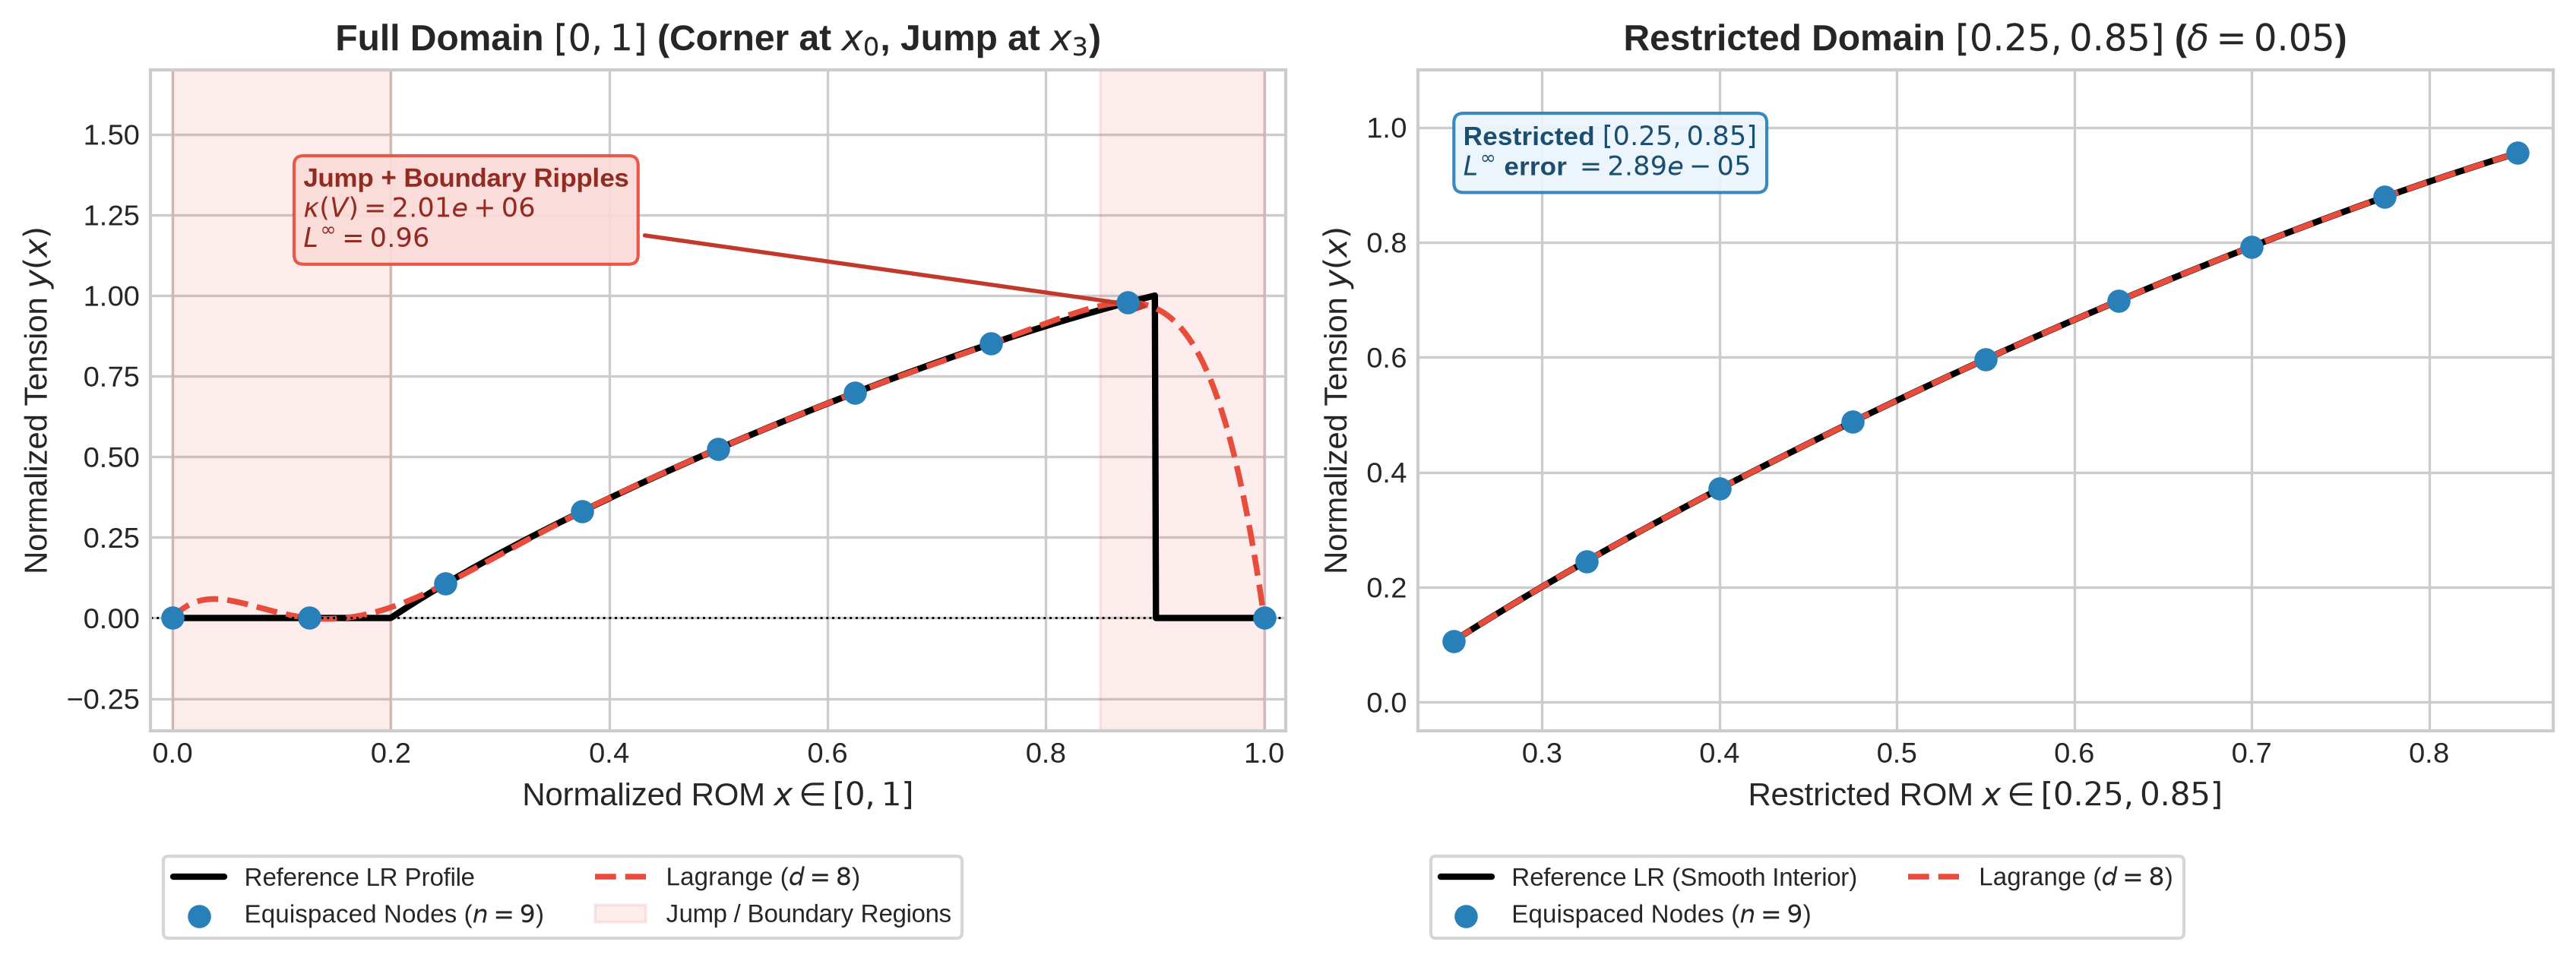
\includegraphics[width=0.96\textwidth]{lagrange_runge.png}
  \caption{Lagrange interpolation ($n=9$ equispaced nodes) on \texttt{LR}. Left: full domain $[0, 1]$, showing the jump-bridge discrepancy at $x_3 = 0.90$ and resting-zone oscillations ($L^\infty = 0.961$, unscaled monomial $\kappa(V) = 2.01 \times 10^6$). Right: restricted domain $[0.25, 0.85]$ ($\delta = 0.05$), isolating smooth interior error ($L^\infty = 2.89 \times 10^{-5}$).}
  \label{fig:runge}
\end{figure*}

Replacing equispaced nodes with Chebyshev--Gauss--Lobatto (CGL) nodes mapped to $[a, b]$,
\begin{equation}
  x_k = a + \frac{b - a}{2}\left(1 - \cos\frac{k\pi}{N - 1}\right), \qquad k = 0, \dots, N-1,
\end{equation}
suppresses the Runge phenomenon and reduces Lebesgue growth to $\Lambda_N = \frac{2}{\pi}\ln N + \mathcal{O}(1)$ (though the unscaled monomial Vandermonde matrix still has $\kappa(V) = 1.02 \times 10^8$ at $N=12$, or $8.46 \times 10^7$ after \texttt{numpy.polyfit} column equilibration). On the smooth interior $[0.25, 0.85]$, CGL achieves $L^\infty = 2.07 \times 10^{-4}$ ($N=6$) and $4.90 \times 10^{-7}$ ($N=12$). Yet on the full physical domain $[0, 1]$, global coupling across the discontinuity at $x_3$ still yields $L^\infty = 0.989$ ($N=6$, $\max = 0.765$) and $0.805$ ($N=12$, overshooting to $1.046$) with negative dips ($y(x) < 0$) in both $[0, 0.2]$ and $(x_3, 1]$ (Fig.~\ref{fig:cgl}), making polynomial interpolation unsuitable for bounded-support exercise profiles.

\begin{figure*}[t]
  \centering
  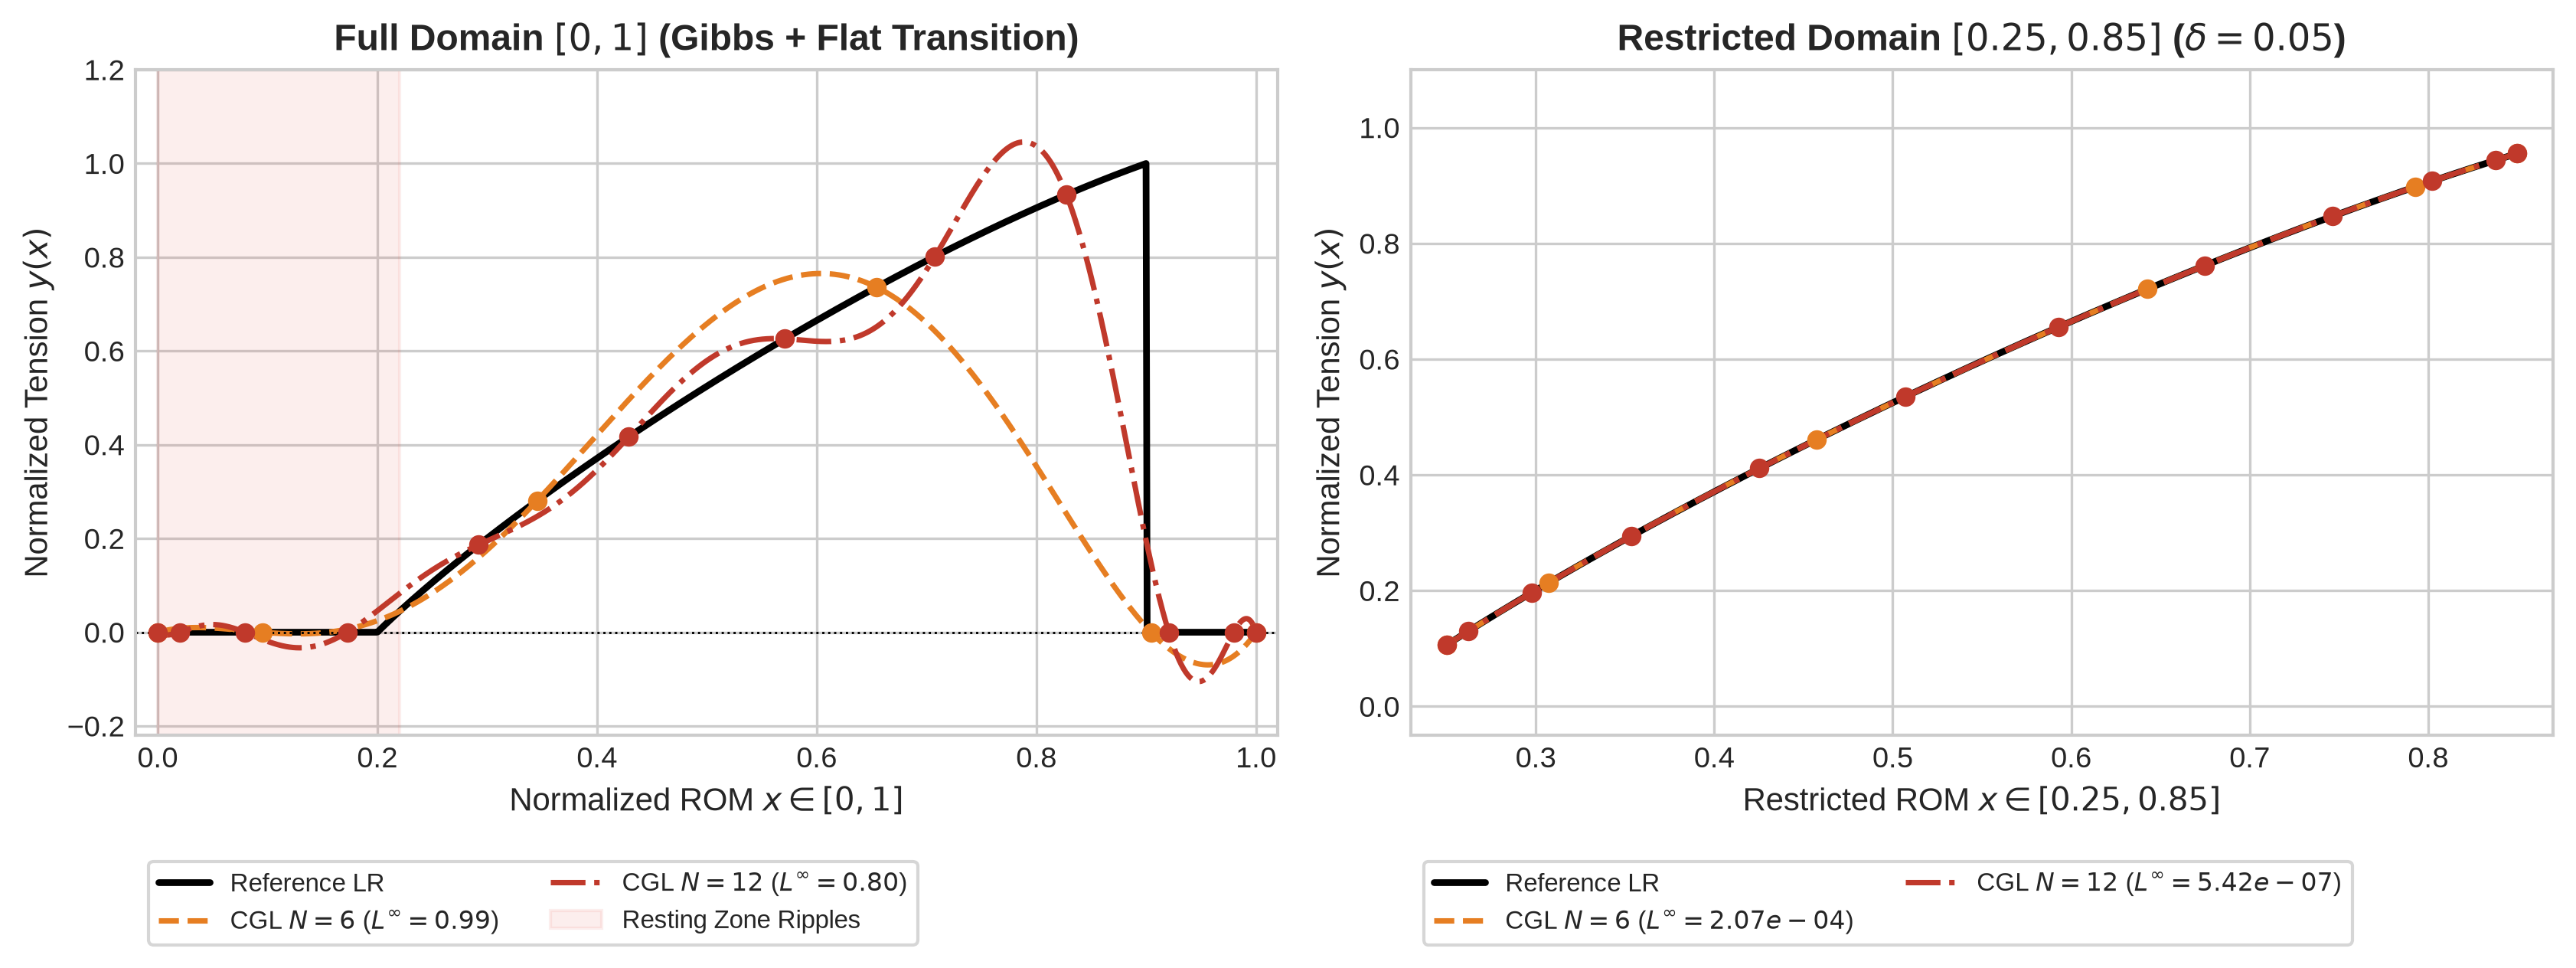
\includegraphics[width=0.96\textwidth]{lagrange_gauss_lobatto.png}
  \caption{Chebyshev--Gauss--Lobatto interpolation ($N=6, 12$) on \texttt{LR}. Left: full domain $[0, 1]$, showing jump error at $x_3$ (overshoot $1.046$ for $N=12$) and negative ripples in $[0, 0.2]$ and $(x_3, 1]$ ($L^\infty = 0.989$ for $N=6$, $0.805$ for $N=12$). Right: restricted domain $[0.25, 0.85]$ ($L^\infty = 2.07 \times 10^{-4}$ and $4.90 \times 10^{-7}$).}
  \label{fig:cgl}
\end{figure*}

\subsection{\texorpdfstring{$C^2$}{C2} Natural Cubic Splines}
Piecewise natural cubic splines partition $[a, b]$ using $N$ knots $a = \tilde{x}_0 < \tilde{x}_1 < \dots < \tilde{x}_{N-1} = b$ into $N-1$ subintervals $[\tilde{x}_k, \tilde{x}_{k+1}]$, enforcing $C^2$ interior continuity and zero boundary curvature $S''(\tilde{x}_0) = S''(\tilde{x}_{N-1}) = 0$. Solving the tridiagonal system $A\mathbf{m} = \mathbf{d}$ via the Thomas algorithm takes $\mathcal{O}(N)$ operations and minimizes $\int_a^b [S''(x)]^2\,dx$ among all $C^2[a, b]$ interpolants passing through $\{(\tilde{x}_k, y_k)\}_{k=0}^{N-1}$ (Holladay's theorem).

On the restricted smooth interior $[0.25, 0.85]$, a uniform $6$-knot natural $C^2$ spline attains $L^\infty = 2.46 \times 10^{-3}$ without oscillation. On the full domain $[0, 1]$, even with knots placed directly at the support boundaries ($N=6$ non-uniform knots $\{0, 0.2, 0.45, 0.75, 0.9, 1\}$), $C^2$ stiffness produces a non-physical negative arch ($y(x) < 0$, down to $-0.040$) across the flat-to-ramp transition $x \in (0, 0.2)$ alongside an overshoot to $1.116$ before $x_3$ and a unit jump discrepancy ($L^\infty = 1.000$ at $x_3^+$) where the continuous interpolant passes through $(0.9, 1.0)$ (Fig.~\ref{fig:spline_over}). Uniform knot refinement does not eliminate negative undershoot across the discontinuity: at $N = 10$ uniform knots, the natural $C^2$ spline still dips below zero ($\min y = -4.29 \times 10^{-4}$, $\max y = 1.043$, $L^\infty = 0.942$), and denser uniform grids ($N \in [15, 50]$) exhibit Gibbs undershoots down to $-0.13$ past $x_3$. Eliminating undershoot requires non-uniform knots tightly bracketing the discontinuities or relaxing continuity to $C^1$ monotone piecewise cubic Hermite interpolation (PCHIP), sacrificing parameter parsimony or $C^2$ curvature (Fig.~\ref{fig:spline_dens}).

\begin{figure*}[t]
  \centering
  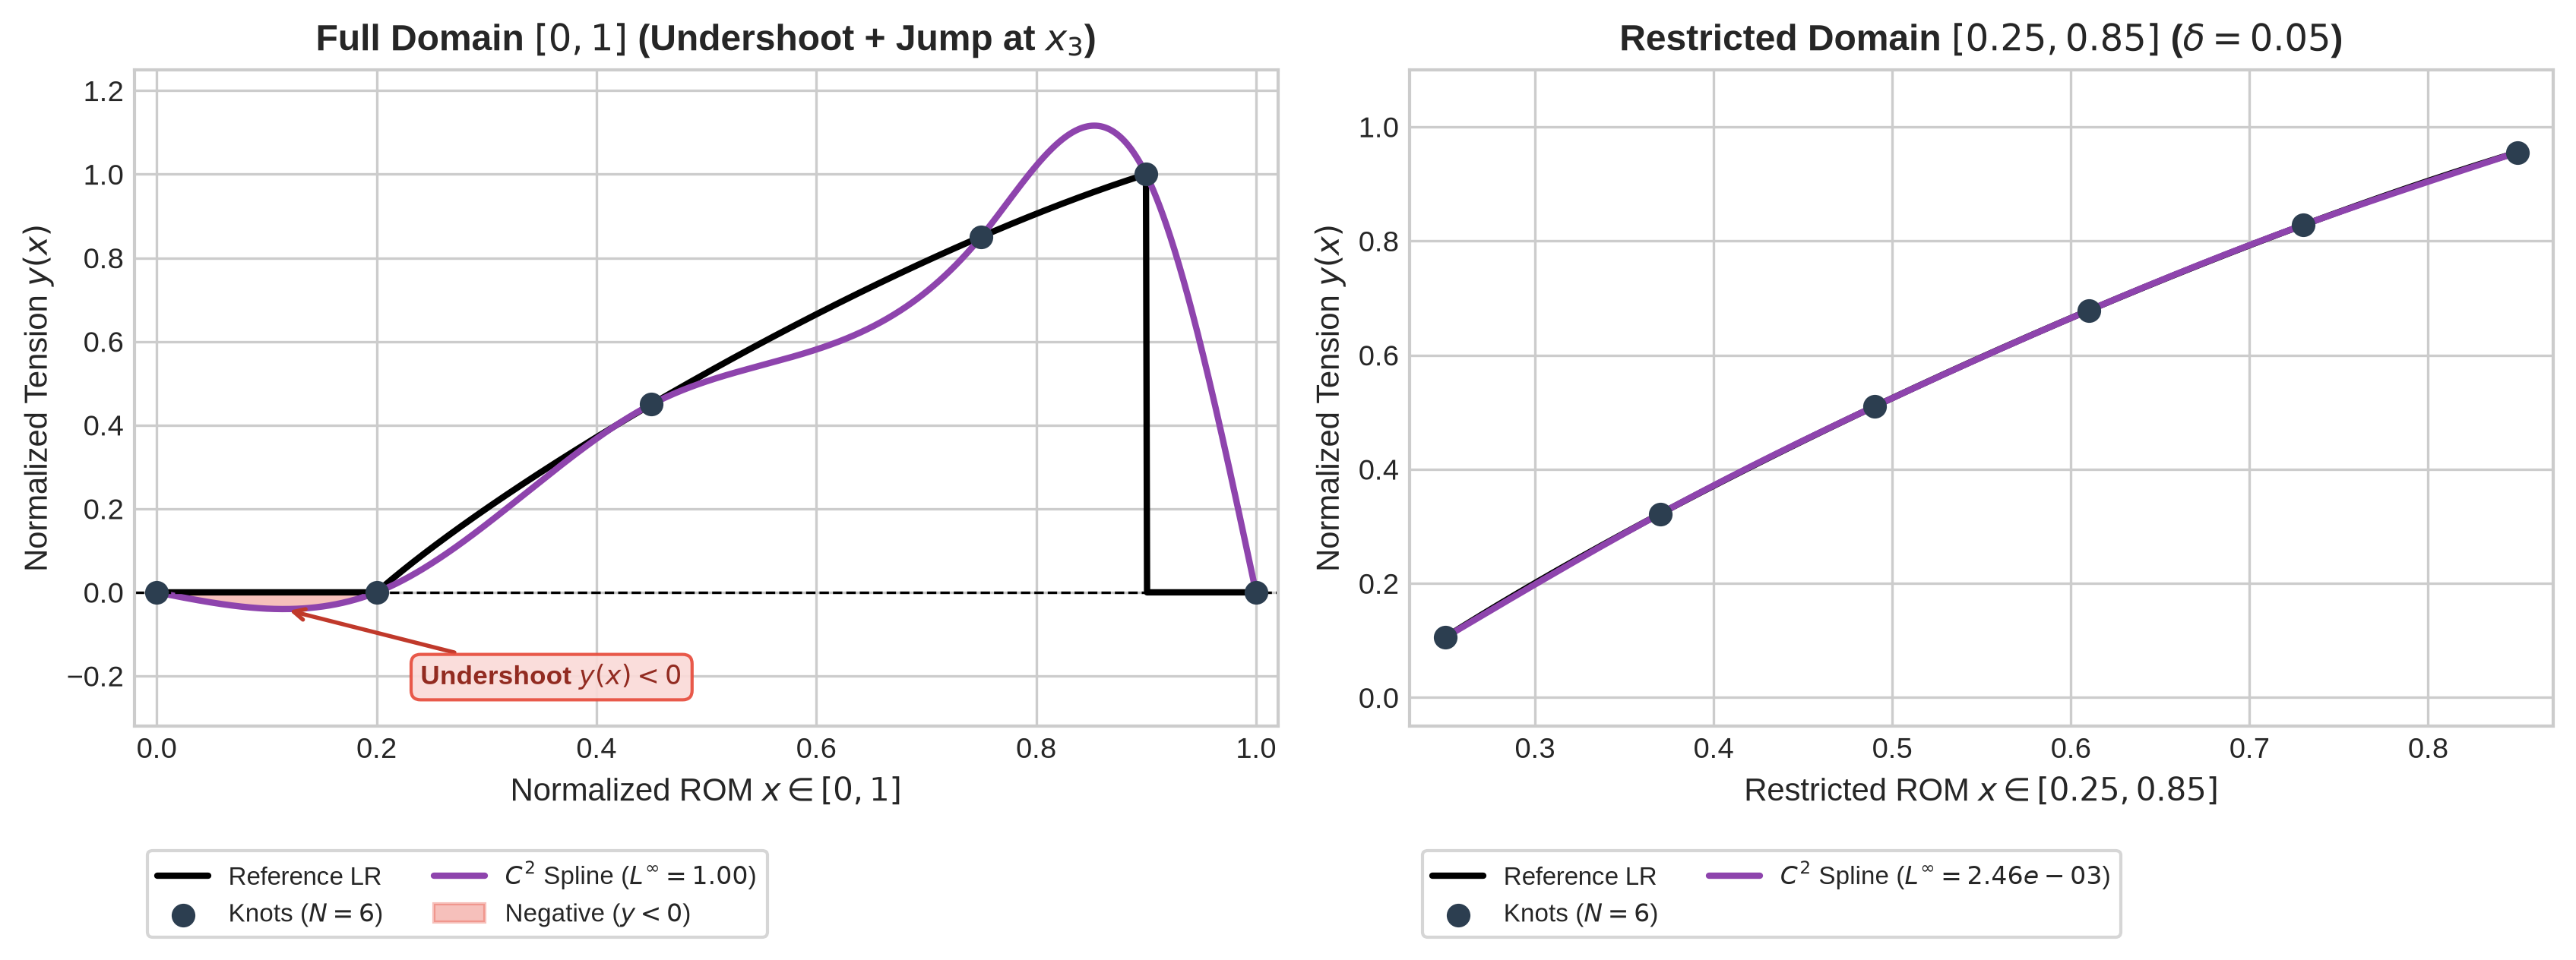
\includegraphics[width=0.96\textwidth]{spline_overshoot.png}
  \caption{Natural $C^2$ cubic spline ($N=6$ knots) on \texttt{LR}. Left: full domain $[0, 1]$ (non-uniform knots placing nodes at $x_0=0.2$ and $x_3=0.9$), exhibiting non-physical negative undershoot ($y(x) < 0$) in $(0, 0.2)$ and unit jump error at $x_3^+$ ($L^\infty = 1.000$). Right: restricted domain $[0.25, 0.85]$ with $6$ uniform knots ($L^\infty = 2.46 \times 10^{-3}$).}
  \label{fig:spline_over}
\end{figure*}

\begin{figure*}[t]
  \centering
  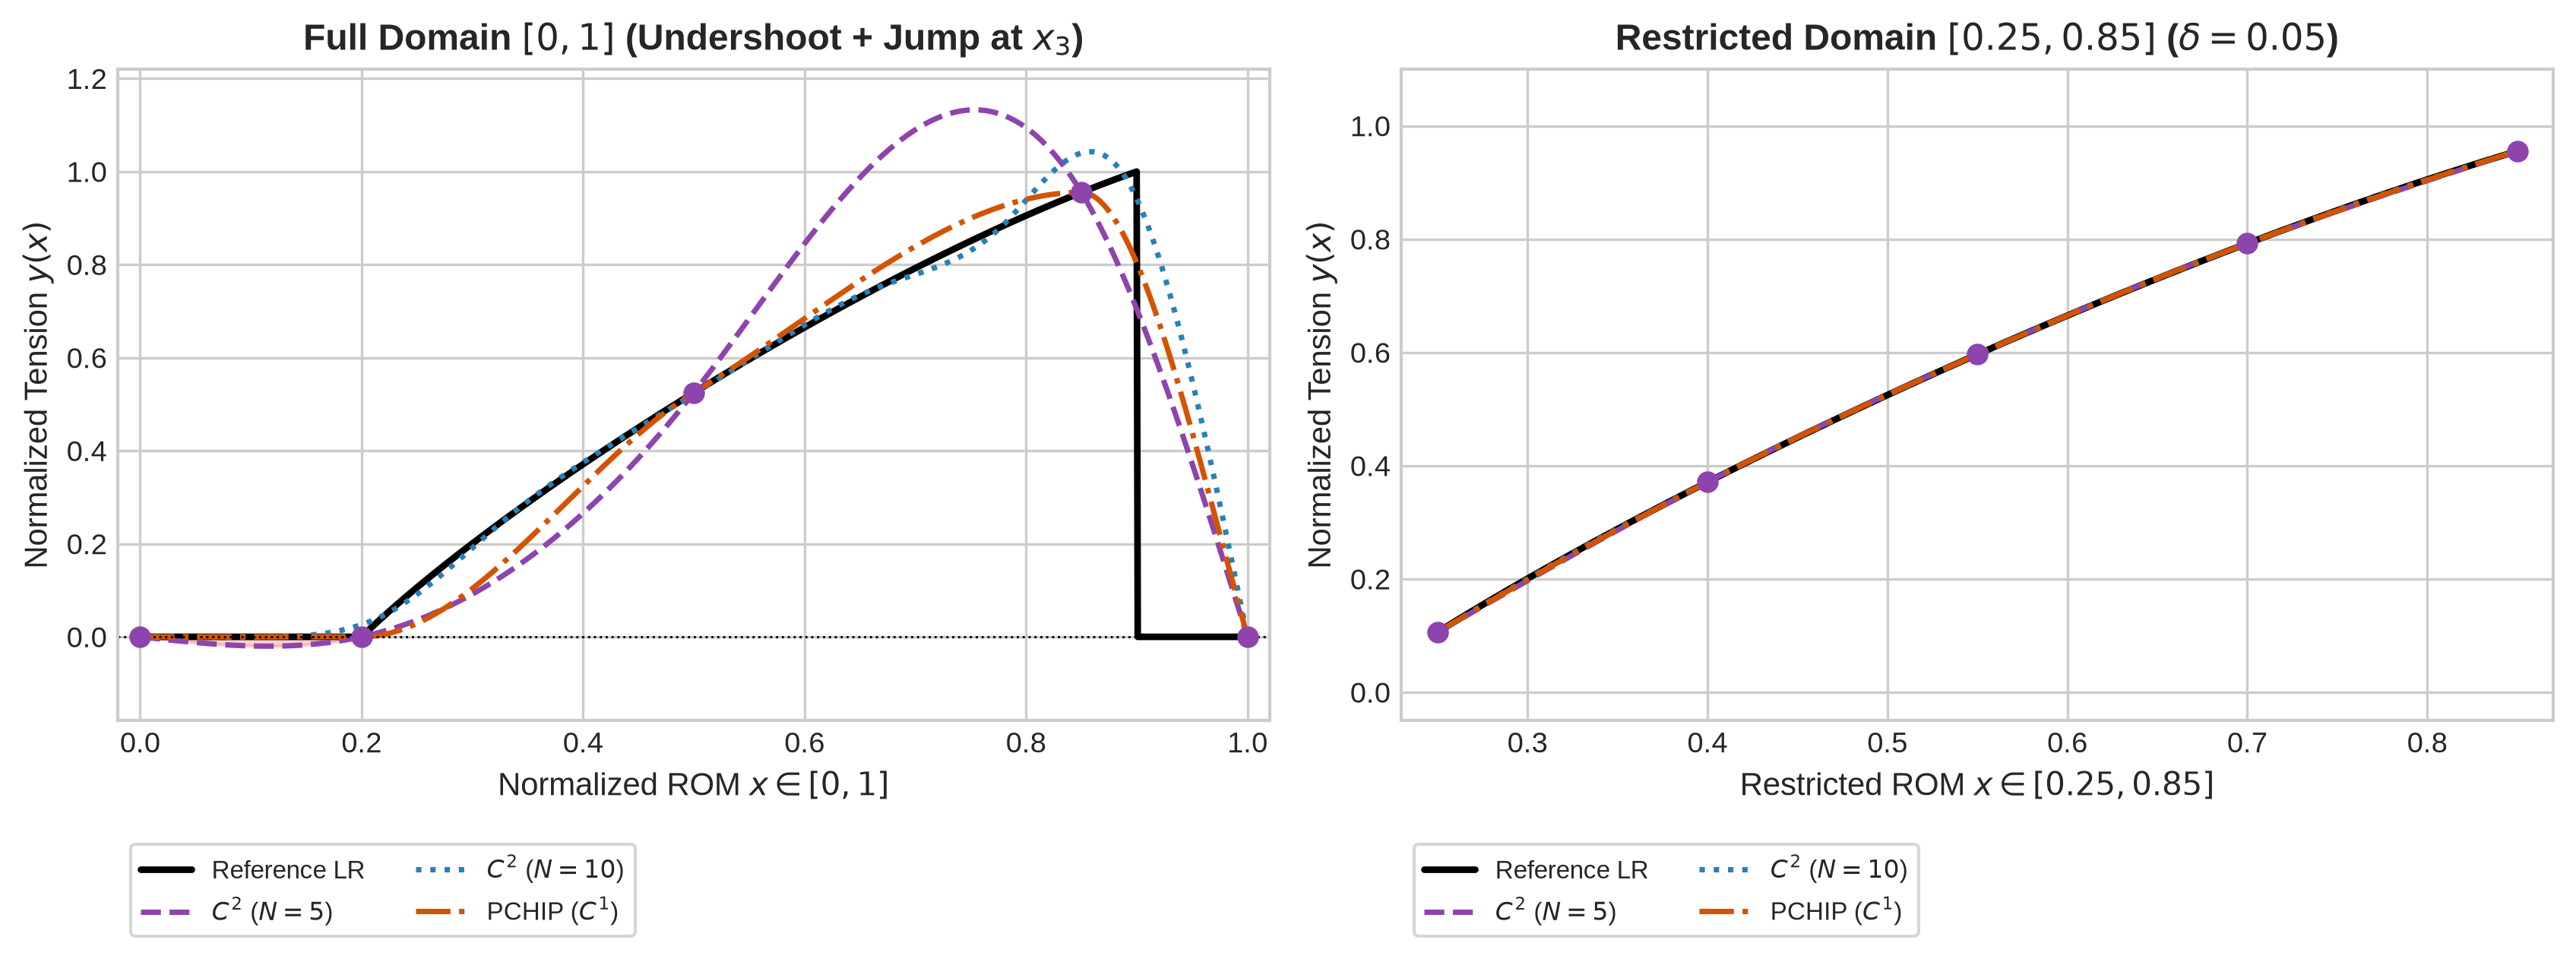
\includegraphics[width=0.96\textwidth]{spline_density.png}
  \caption{Spline trade-off on \texttt{LR}. Left: full domain $[0, 1]$ (non-uniform $N=5$ knots including $x_0=0.2$ still undershoots, uniform $N=10$ inflates user knots, PCHIP on $N=5$ reduces to $C^1$). Right: restricted domain $[0.25, 0.85]$ (uniform knots) showing smooth interior agreement.}
  \label{fig:spline_dens}
\end{figure*}

\subsection{Cubic B\'ezier Curves, Monotonicity, and Bernstein Guarantees}
In \texttt{BezierProfile} (\texttt{models.py}), each active tension profile over $[x_0, x_3] \subseteq [0, 1]$ is defined parametrically by four absolute 2D control points $\mathbf{P}_i = (x_i, y_i)^\top$ with $x_i \in [0, 1]$ and $y_i \ge 0$, $i \in \{0, 1, 2, 3\}$ (default catalog and interactive editor profiles lie in $[0, 1]^2$), in the cubic Bernstein basis (and $y(x) = 0$ for $x \notin [x_0, x_3]$):
\begin{equation}
  \mathbf{P}(t) = \begin{pmatrix} x(t) \\ y(t) \end{pmatrix} = \sum_{i=0}^{3} \mathbf{P}_i B_{i,3}(t), \qquad t \in [0, 1],
  \label{eq:bezier}
\end{equation}
where $B_{i,3}(t) = \binom{3}{i} t^i (1 - t)^{3-i}$. Explicitly, both components share the same convex combination:
\begin{align}
  x(t) &= (1-t)^3 x_0 + 3(1-t)^2 t\, x_1 + 3(1-t) t^2\, x_2 + t^3 x_3, \label{eq:bx} \\
  y(t) &= (1-t)^3 y_0 + 3(1-t)^2 t\, y_1 + 3(1-t) t^2\, y_2 + t^3 y_3. \label{eq:by}
\end{align}

\begin{theorem}[Convex Hull Non-Negativity]
For all $t \in [0, 1]$, the cubic Bernstein polynomials satisfy $B_{i,3}(t) \ge 0$ and form a partition of unity $\sum_{i=0}^{3} B_{i,3}(t) = \bigl((1-t) + t\bigr)^3 \equiv 1$. Consequently, $\mathbf{P}(t) \in \mathrm{Conv}(\{\mathbf{P}_0, \mathbf{P}_1, \mathbf{P}_2, \mathbf{P}_3\})$, and if $y_i \ge 0$ for all $i \in \{0, 1, 2, 3\}$, then $y(t) \ge 0$ for every $t \in [0, 1]$.
\end{theorem}

\begin{proof}
Since $t \ge 0$ and $1 - t \ge 0$ on $[0, 1]$, each $B_{i,3}(t) \ge 0$. By the binomial theorem, $\sum_{i=0}^3 \binom{3}{i} t^i (1-t)^{3-i} = 1$, so $y(t) = \sum_{i=0}^3 B_{i,3}(t) y_i$ is a convex combination of $\{y_i\}$ and satisfies $\min_i y_i \le y(t) \le \max_i y_i$. Setting $y_i \ge 0$ guarantees $y(t) \ge 0$ identically.
\end{proof}

Geometrically, $\mathbf{P}(t)$ admits De Casteljau's division-free recursive convex interpolation construction (Fig.~\ref{fig:decasteljau}):
\begin{align*}
  \mathbf{Q}_i(t) &= (1-t)\mathbf{P}_i + t\mathbf{P}_{i+1}, & i &\in \{0, 1, 2\}, \\
  \mathbf{R}_i(t) &= (1-t)\mathbf{Q}_i(t) + t\mathbf{Q}_{i+1}(t), & i &\in \{0, 1\}, \\
  \mathbf{P}(t) &= (1-t)\mathbf{R}_0(t) + t\mathbf{R}_1(t),
\end{align*}
where $\mathbf{R}_0(t)\mathbf{R}_1(t)$ gives the exact tangent direction and endpoints obey $\mathbf{P}'(0) = 3(\mathbf{P}_1 - \mathbf{P}_0)$ and $\mathbf{P}'(1) = 3(\mathbf{P}_3 - \mathbf{P}_2)$; \texttt{models.py::BezierProfile.get\_curve} evaluates~\eqref{eq:bx}--\eqref{eq:by} directly over uniform $t$ in $\mathcal{O}(1)$ per-point time, whereas physical-ROM queries in \texttt{solve\_y}, \texttt{helpers.js::solveBezierY}, and \texttt{solver.js} run bounded bisection (at most $30$ evaluations of $x(t)$ plus $1$ final evaluation of $y(t)$, $\mathcal{O}(1)$ in control-point count).

While \texttt{BezierProfile.get\_curve} evaluates~\eqref{eq:bx}--\eqref{eq:by} directly over $t \in [0, 1]$, querying tension at a physical ROM coordinate $x_{\mathrm{target}} \in [x_0, x_3]$ requires inverting $x(t^*) = x_{\mathrm{target}}$ (implemented in \texttt{models.py::BezierProfile.solve\_y} and \texttt{helpers.js::solveBezierY}). Requiring $x_0 < x_1 < x_2 < x_3$ is a clean \emph{sufficient} (though not necessary) condition for strict monotonicity: since $x'(t) = 3(1-t)^2(x_1 - x_0) + 6(1-t)t(x_2 - x_1) + 3t^2(x_3 - x_2)$ is $3$ times a convex combination of strictly positive increments, $x'(t) > 0$ on $[0, 1]$ and $t^*$ is unique. This invariant (together with $0 \le x_0 < x_1 < x_2 < x_3 \le 1$ and $y_i \ge 0$) is enforced at load and edit time in \texttt{BezierProfile.\_\_post\_init\_\_}, \texttt{parser.py}/\texttt{parser.js} (\texttt{override:} handling), \texttt{WorkoutSolver} (\texttt{solver.js}), \texttt{solveBezierY}, and \texttt{BezierEditor.jsx}, and holds across all 61 exercises in \texttt{defaultExercises.json}. After $K$ bisection updates on $t \in [0, 1]$ (without early exit),
\begin{equation}
\begin{gathered}
  \lvert t^{(K)} - t^* \rvert \le 2^{-(K+1)}, \\
  \lvert x(t^{(K)}) - x_{\mathrm{target}} \rvert \le 2^{-(K+1)} \max_{[0,1]} \lvert x'(t) \rvert.
\end{gathered}
\end{equation}
Both \texttt{solve\_y} and \texttt{solveBezierY} run up to $K = 30$ iterations, exiting early only when \emph{both} $\lvert x(t^{(k)}) - x_{\mathrm{target}} \rvert < 10^{-6}$ \emph{and} the bracket width satisfies $u_k - \ell_k < 10^{-6}$. Because $t^{(k)}$ is the bracket midpoint, this dual criterion guarantees $\lvert t^{(k)} - t^* \rvert < 5 \times 10^{-7}$ and $\lvert y(t^{(k)}) - y(t^*) \rvert \le \frac{1}{2}\cdot 10^{-6}\max_{[0,1]} \lvert y'(t) \rvert$ uniformly even when $x'(t^*)$ is arbitrarily small. Fig.~\ref{fig:bernstein}, Fig.~\ref{fig:comparison}, and Table~\ref{tab:comparison} summarize the Bernstein basis and method comparison.

\begin{figure}[t]
  \centering
  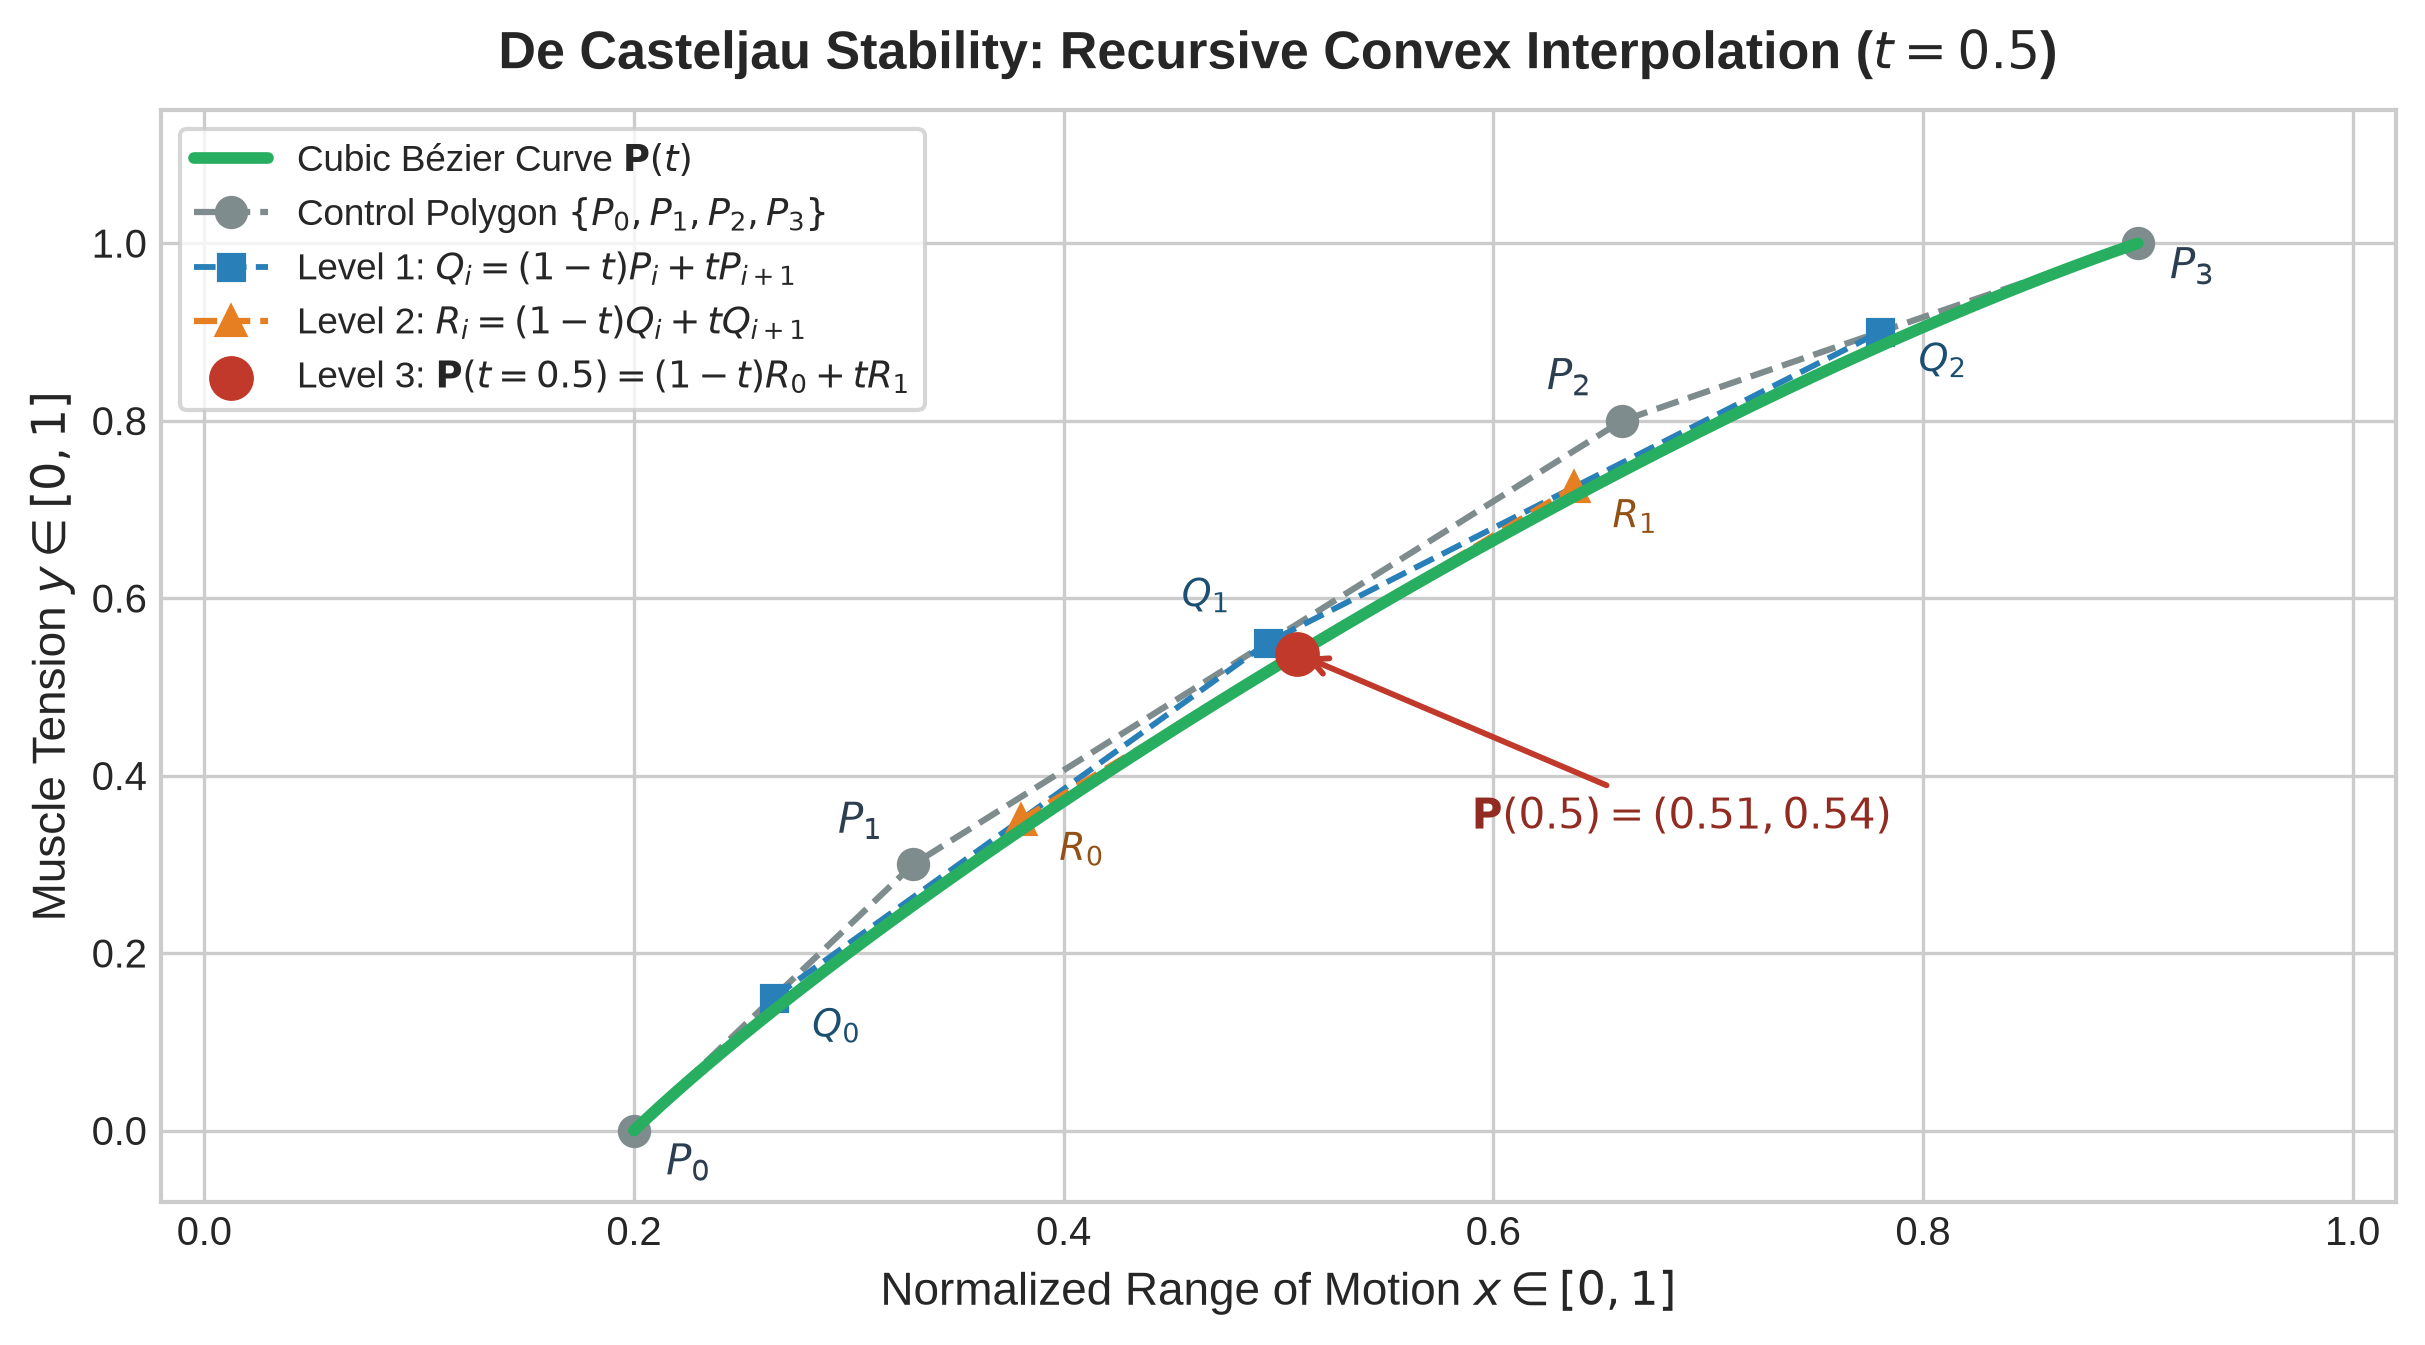
\includegraphics[width=\linewidth]{de_casteljau.png}
  \caption{De Casteljau geometric construction at $t = 0.5$ on \texttt{LR}, requiring six division-free convex linear interpolations in $\mathcal{O}(1)$ time.}
  \label{fig:decasteljau}
\end{figure}

\begin{figure*}[t]
  \centering
  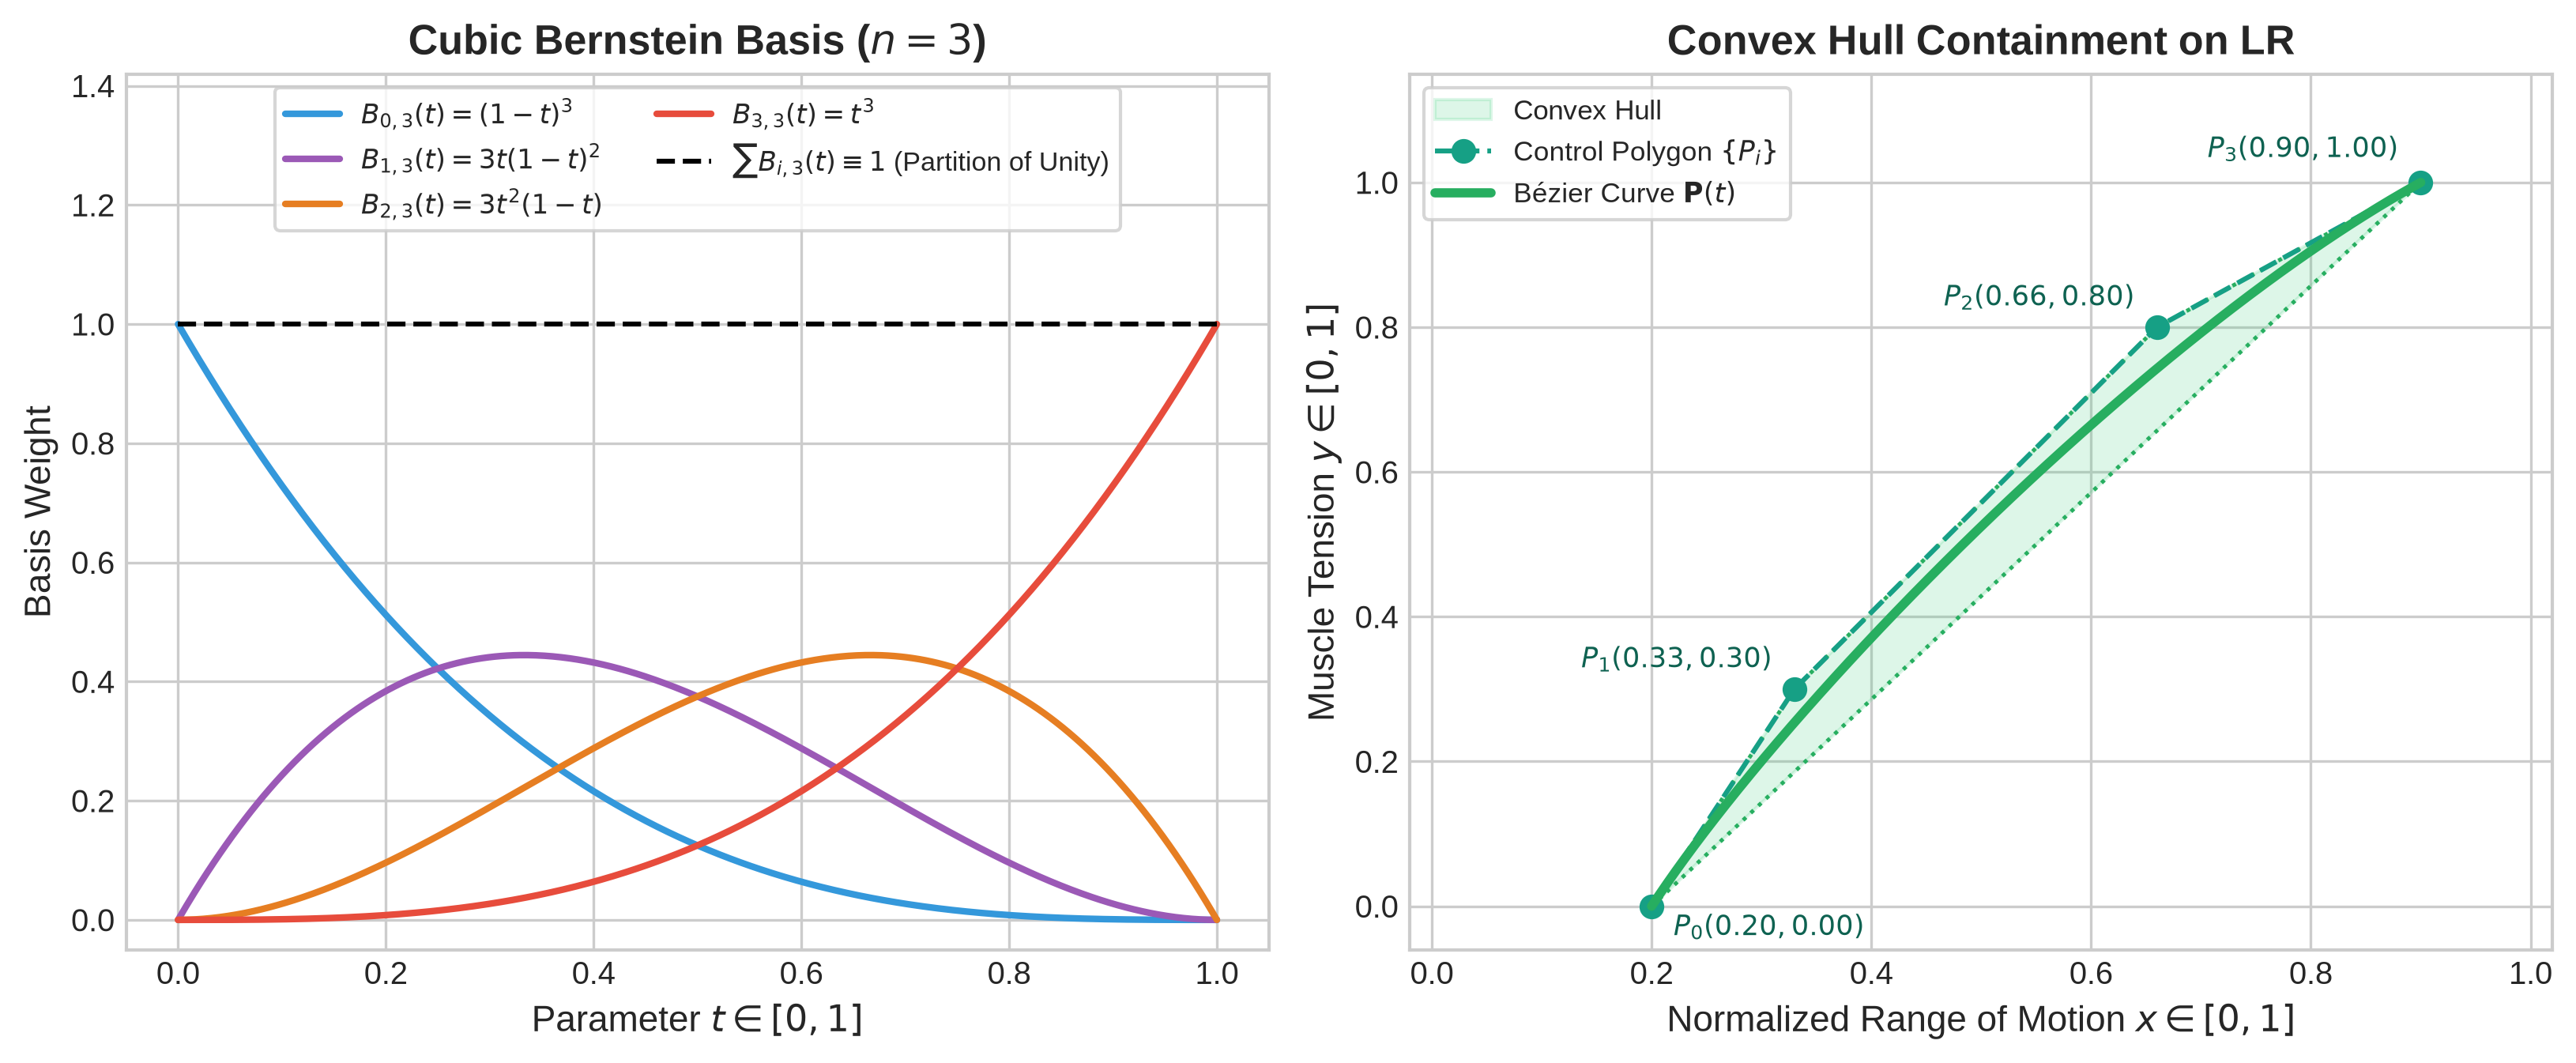
\includegraphics[width=0.92\textwidth]{bezier_bernstein.png}
  \caption{Left: Cubic Bernstein basis polynomials $B_{i,3}(t)$ verifying $\sum_{i=0}^3 B_{i,3}(t) \equiv 1$. Right: Resulting \texttt{LR} curve enclosed within the convex hull of its four control points (with endpoints $\mathbf{P}_0, \mathbf{P}_3$ on the hull boundary).}
  \label{fig:bernstein}
\end{figure*}

\begin{figure*}[t]
  \centering
  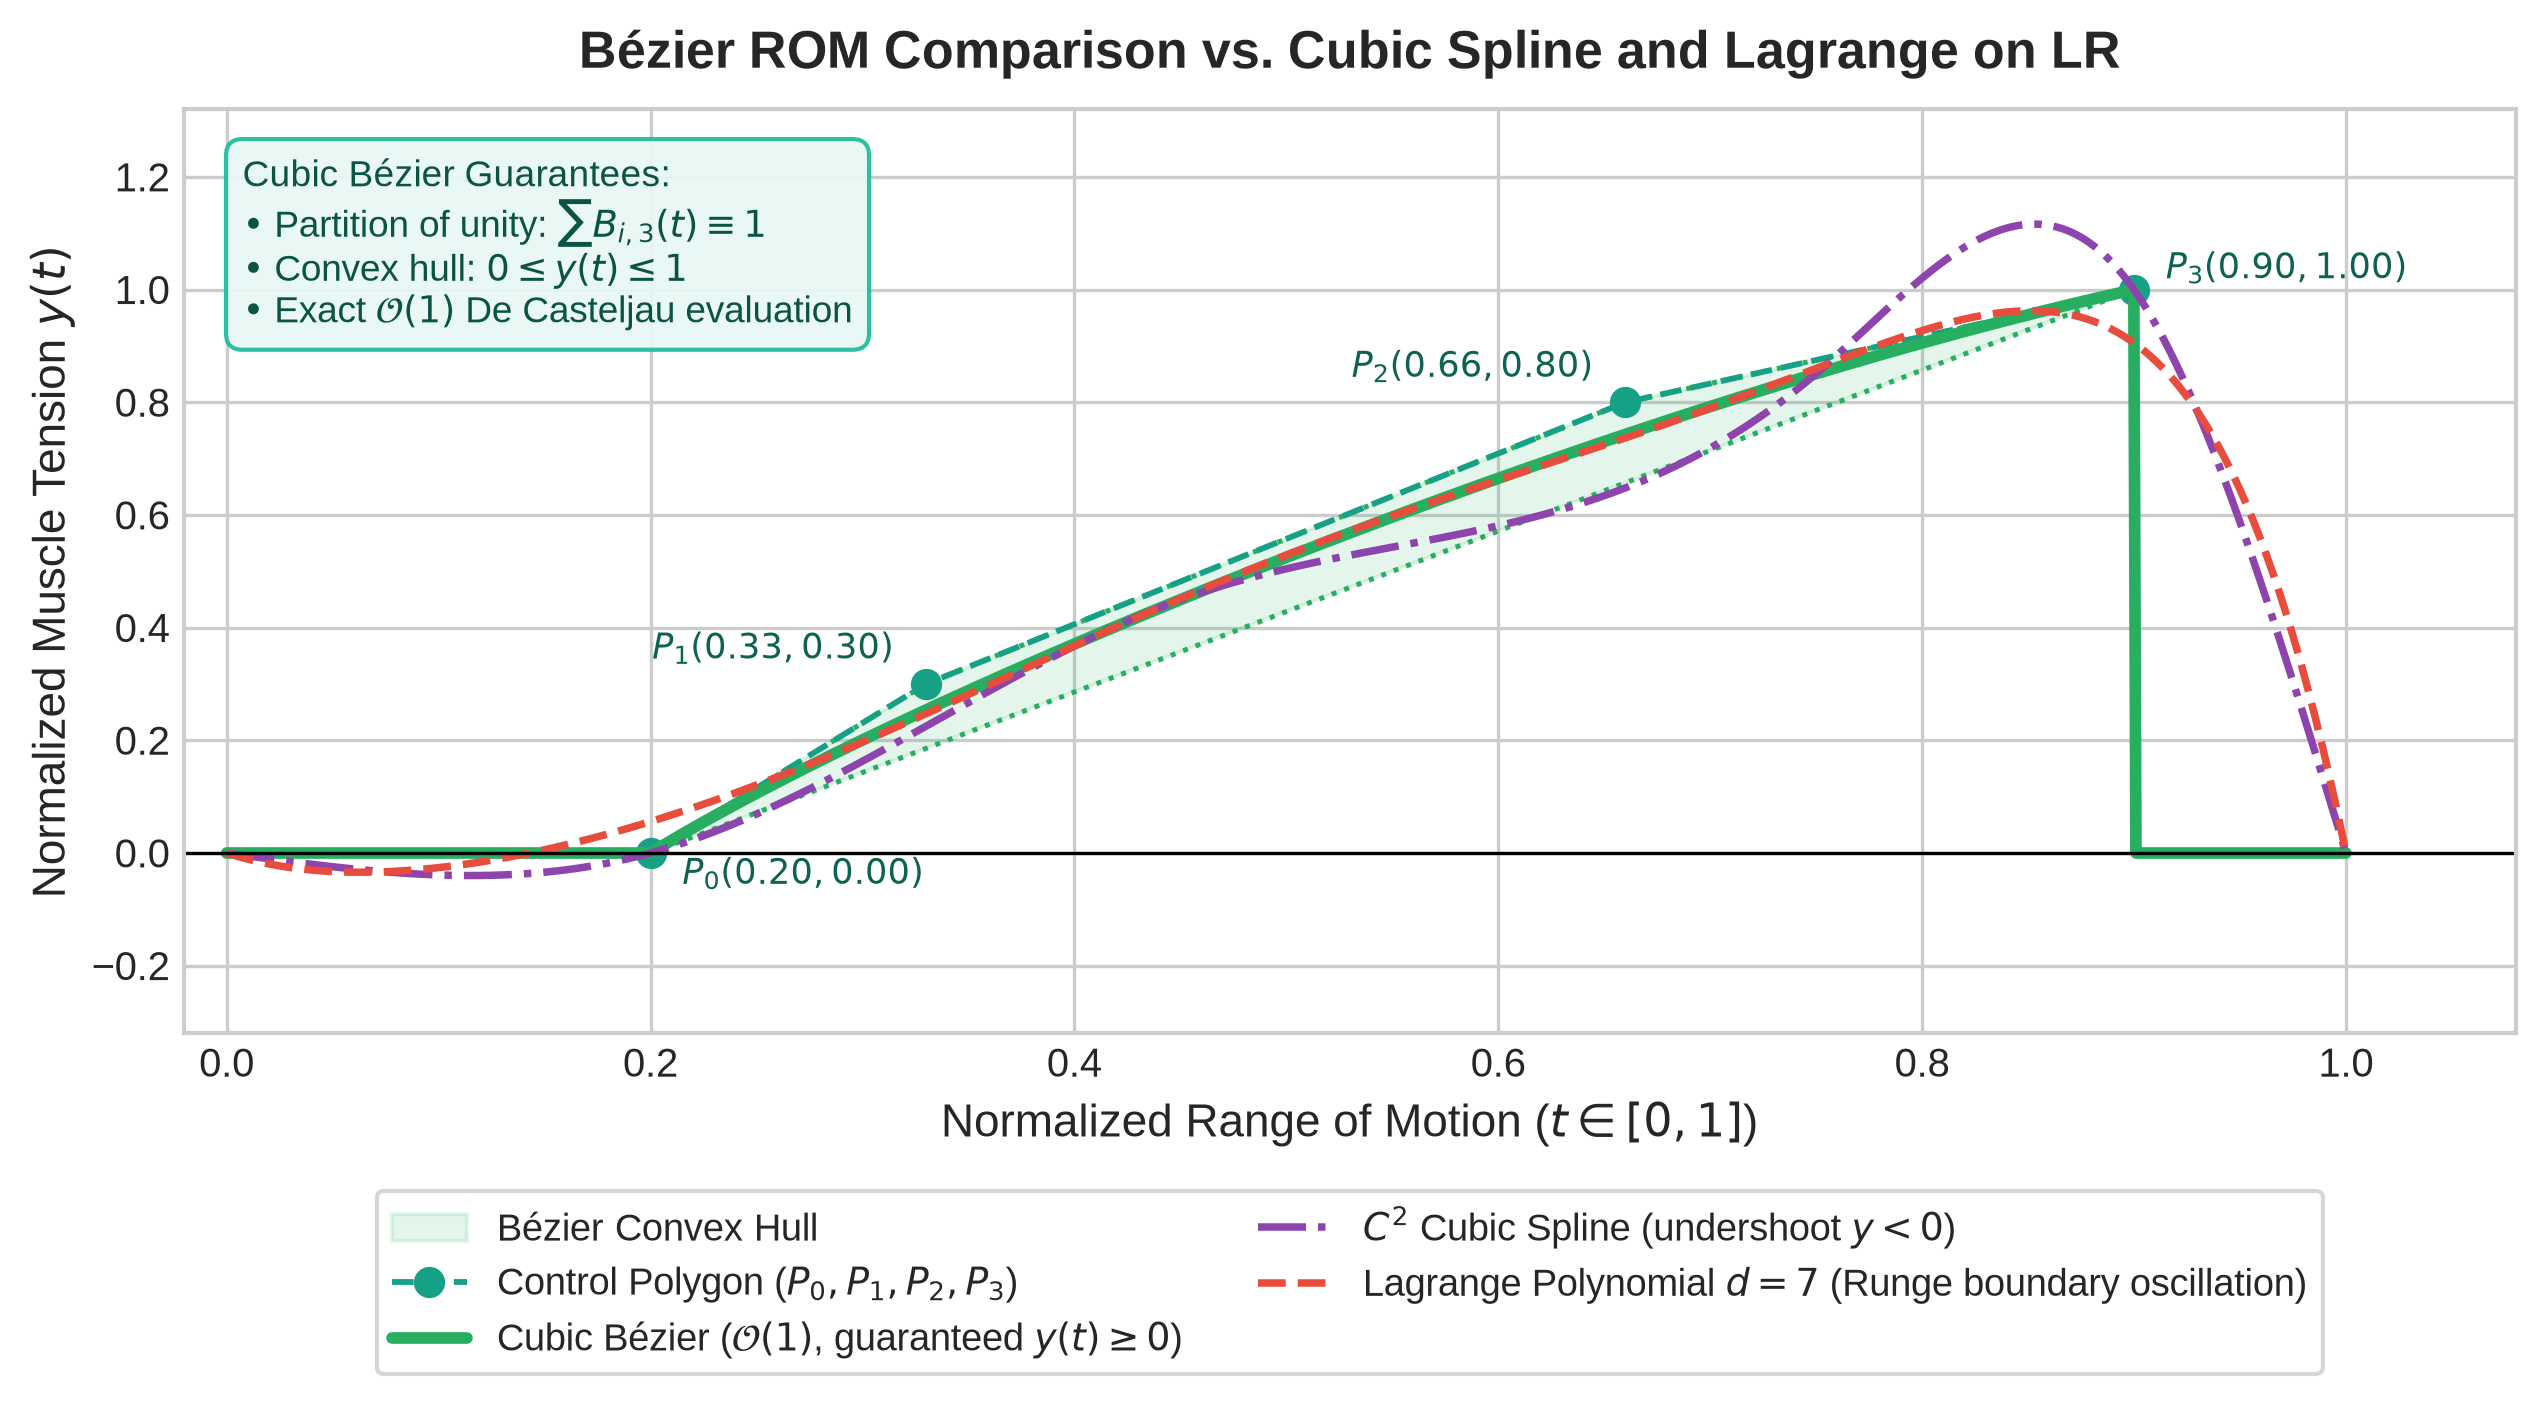
\includegraphics[width=0.96\textwidth]{bezier_comparison.png}
  \caption{Synoptic comparison on \texttt{LR}. Left: full domain $[0, 1]$, showing $C^2$ spline overshoot ($1.116$) and jump error at $x_3 = 0.90$ alongside Lagrange $d=7$ jump-bridge discrepancy ($\max = 0.963 < 1.0$). Right: restricted domain $[0.25, 0.85]$ ($\delta = 0.05$), isolating smooth interior errors ($L^\infty = 6.29 \times 10^{-5}$ for Lagrange $d=7$, $2.46 \times 10^{-3}$ for $N=6$ $C^2$ spline).}
  \label{fig:comparison}
\end{figure*}

\begin{table}[t]
  \centering
  \caption{Numerical properties of ROM tension approximations.}
  \label{tab:comparison}
  \scriptsize
  \setlength{\tabcolsep}{3.5pt}
  \begin{tabular}{@{}lcccc@{}}
    \toprule
    \textbf{Method} & \textbf{Params} & \textbf{Query Cost} & \textbf{$y(x)\!\ge\!0$} & \textbf{Support $[x_0,x_3]$} \\
    \midrule
    Lagrange (Equi.) & $n$ nodes & $\mathcal{O}(n)$ (bary.) & No & Runge + $x_3$ jump \\
    Lagrange (CGL) & $N$ nodes & $\mathcal{O}(N)$ (bary.) & No & Ripples + $x_3$ jump \\
    Natural $C^2$ Spline & $N$ knots & $\mathcal{O}(\log N)$ & No & Dip + $x_3$ jump \\
    \textbf{Cubic B\'ezier} & \textbf{4 pts} & $\bm{\mathcal{O}(1)}$ & \textbf{Yes} & \textbf{Exact $[x_0,x_3]$} \\
    \bottomrule
  \end{tabular}
\end{table}

\subsection{Exact Parametric Quadrature vs.\ Trapezoidal Discretization}
To conserve muscle contribution magnitude $M_{e,m}$ under arbitrary control-point shapes, consider integrating $y\,dx$ across $[x_0, x_3]$. Sampling $t_k = k/(R-1)$ ($R = 50$, $h = 1/(R-1)$) with $\Delta x_k = x(t_{k+1}) - x(t_k)$ via the composite trapezoidal rule gives
\begin{equation}
  I_{\mathrm{trap}} = \sum_{k=0}^{R-2} \frac{y(t_k) + y(t_{k+1})}{2}\,\Delta x_k.
\end{equation}
Because $t_k$ is uniform while $x(t_k)$ is \emph{non-uniformly spaced}, the classical uniform-grid formula $-\frac{(x_3 - x_0)^3}{12(R-1)^2} y''(\xi)$ does \emph{not} apply. Under strict monotonicity ($x_0 < x_1 < x_2 < x_3$, ensuring $\Delta x_k > 0$ and $y \circ x^{-1} \in C^\infty([x_0, x_3])$), expanding $y(x)$ symmetrically around each spatial midpoint $m_k = \frac{1}{2}\bigl(x(t_k) + x(t_{k+1})\bigr)$ cancels all odd-degree terms in the single-interval error $e_k = \int_{x(t_k)}^{x(t_{k+1})} y(x)\,dx - \frac{y(t_k) + y(t_{k+1})}{2}\Delta x_k$, giving
\begin{equation}
\begin{aligned}
  E_{\mathrm{trap}} &= I_{\mathrm{exact}} - I_{\mathrm{trap}} \\
  &= -\frac{1}{12} \sum_{k=0}^{R-2} \frac{d^2y}{dx^2}(m_k)\,(\Delta x_k)^3 + \mathcal{O}\!\left(\sum_{k=0}^{R-2} (\Delta x_k)^5\right).
\end{aligned}
\end{equation}
Since $m_k = x(t_{k+1/2}) + \mathcal{O}(h^2)$, $\Delta x_k = h \dot{x}(t_{k+1/2}) + \mathcal{O}(h^3)$, and $\frac{d^2y}{dx^2} = \bigl(\ddot{y}(t)\dot{x}(t) - \dot{y}(t)\ddot{x}(t)\bigr)/(\dot{x}(t))^3$ (dots denoting $d/dt$), the midpoint Riemann sum has $\mathcal{O}(h^2)$ quadrature error and yields the $\mathcal{O}(h^2)$ parametric asymptotic expansion
\begin{equation}
  E_{\mathrm{trap}} = -\frac{h^2}{12} \int_0^1 \bigl(\ddot{y}(t)\dot{x}(t) - \dot{y}(t)\ddot{x}(t)\bigr)\,dt + \mathcal{O}(h^4),
\end{equation}
which equals $2.31 \times 10^{-5}$ on \texttt{LR} ($R=50$). By contrast, applying a uniform-$x$ trapezoidal rule on $[0, 1]$ integrates across the boundary discontinuity at $x_3$ on \texttt{LR} (and across jump discontinuities at both $x_0$ and $x_3$ on \texttt{Deadlift}/\texttt{RDL} \emph{Erectors}), degrading convergence to $\mathcal{O}(h)$ with grid-alignment sensitivity: at $R = 50$ ($\Delta x = 1/49$), the relative error is $2.06\%$ on \texttt{LR} and $1.97\%$ on \texttt{Deadlift}/\texttt{RDL} \emph{Erectors}, jumping to $2.51\%$ and $9.52\%$ at $R = 51$ ($\Delta x = 1/50 = 0.02$, matching \texttt{DashboardTab.jsx}'s step size where $x = 0.4, 0.6, 0.9$ align directly with grid nodes). Because $g(t) = y(t)x'(t)$ is a degree-5 polynomial on $[0, 1]$, 3-point Gauss--Legendre quadrature integrates $I_{\mathrm{exact}} = \int_0^1 y(t)x'(t)\,dt$ \emph{exactly} to machine precision ($2(3)-1 = 5$):
\begin{equation}
  I_{\mathrm{GL3}} = \sum_{k=1}^{3} w_k\, y(t_k)\, x'(t_k), \qquad
  t_k = \frac{1 + \xi_k}{2},\; w_k = \frac{\tilde{w}_k}{2},
  \label{eq:gl3}
\end{equation}
with standard nodes $\xi_k \in \{-\sqrt{3/5}, 0, \sqrt{3/5}\}$ and weights $\tilde{w}_k \in \{5/9, 8/9, 5/9\}$. For each $m \in \mathcal{M}_e$, the area-normalized tension density is defined on $[0, 1]$ as
\begin{equation}
  B_{e,m}(x) =
  \begin{cases}
    \dfrac{M_{e,m}}{I_{\mathrm{GL3},e,m}}\, y_{e,m}\bigl(x_{e,m}^{-1}(x)\bigr), &
    \begin{aligned}[t]
      &x \in [x_{0,e,m}, x_{3,e,m}] \\
      &\text{and } I_{\mathrm{GL3},e,m} > 0,
    \end{aligned} \\
    0, & \text{otherwise},
  \end{cases}
  \label{eq:normalized_density}
\end{equation}
and $B_{e,m}(x) \equiv 0$ for $m \notin \mathcal{M}_e$. \texttt{BezierProfile.exact\_area()} and \texttt{helpers.js::bezierArea} compute $I_{\mathrm{GL3}}$ via~\eqref{eq:gl3}, while \texttt{BezierProfile.get\_physical\_curve()}, \texttt{solver.js}, and \texttt{DashboardTab.jsx} (which samples $51$ ROM points $i/50$ versus $50$ points $i/49$ in the solver) all evaluate~\eqref{eq:normalized_density}, eliminating quadrature drift across both backend and frontend.

\section{Physiological Dynamics \texorpdfstring{\&}{and} Optimization}
\label{sec:metrics_solver}

\subsection{Effective Volume, Dynamic TUT, and CNS Fatigue}
In \texttt{constants.py} and \texttt{models.py} (\texttt{SetData}), each set contains $n_b$ base repetitions, $n_a$ assisted repetitions ($\alpha_{\mathrm{ass}} = 0.5$), and $n_p$ partial repetitions ($\alpha_{\mathrm{part}} = 0.33$). Both \texttt{parser.py}/\texttt{parser.js} and \texttt{metrics.py} clamp $\mathrm{RPE}$ to $[0.0, 10.0]$ (defaulting omitted set RPE to $9.0$, with \texttt{SetData} rejecting negative repetition counts or $\mathrm{RPE} < 0$); by contrast, the simulated-annealing solver in \texttt{solver.py}/\texttt{solver.js} restricts candidate RPE values to $[5.0, 10.0]$ during mutation as a search-space restriction. Total and HTMU-effective repetitions are:
\begin{align}
  n_{b,\mathrm{eff}} &= \min\bigl(n_b, \max(0, \mathrm{RPE} - 4.0)\bigr), \\
  R_{\mathrm{tot}} &= n_b + \alpha_{\mathrm{ass}} n_a + \alpha_{\mathrm{part}} n_p, \\
  R_{\mathrm{eff}} &= n_{b,\mathrm{eff}} + \alpha_{\mathrm{ass}} n_a + \alpha_{\mathrm{part}} n_p.
\end{align}
Base repetitions recruit high-threshold motor units when $\mathrm{RIR} < 6$ ($\mathrm{RPE} > 4.0$). Note that logbook-level summaries (\texttt{SetData}, \texttt{metrics.py}) credit $\alpha_{\mathrm{ass}} n_a$ and $\alpha_{\mathrm{part}} n_p$ unconditionally at the set level, whereas the mesocycle solver (\S\ref{subsec:solver}) specifically restricts $n_p$ to stretched-ROM partials on $[0, 0.3333]$ with $\mathrm{RPE} \ge 9.0$.

In \texttt{metrics.py} (\texttt{calculate\_set\_tuts}), given execution tempo $(c, p_s, e, p_l)$ (default $1\text{-}0\text{-}2\text{-}0\,\text{s}$) with nominal duration $\tau_0 = c + p_s + e + p_l$, each base repetition $j \in \{0, \dots, n_b - 1\}$ experiences instantaneous $\mathrm{RIR}_j = (10.0 - \mathrm{RPE}) + (n_b - 1 - j)$ and concentric slowdown $\Delta c(\mathrm{RIR}_j)$:
\begin{equation}
  \Delta c(\mathrm{RIR}_j) =
  \begin{cases}
    1.60\,\text{s}, & \mathrm{RIR}_j < 1.0, \\
    1.00\,\text{s}, & 1.0 \le \mathrm{RIR}_j < 2.0, \\
    0.60\,\text{s}, & 2.0 \le \mathrm{RIR}_j < 3.0, \\
    0.35\,\text{s}, & 3.0 \le \mathrm{RIR}_j < 4.0, \\
    0.15\,\text{s}, & 4.0 \le \mathrm{RIR}_j < 5.0, \\
    0.00\,\text{s}, & \mathrm{RIR}_j \ge 5.0,
  \end{cases}
\end{equation}
yielding per-rep TUT $\tau_j = \tau_0 + \Delta c(\mathrm{RIR}_j)$ for base reps, $\tau_0$ for assisted reps, and $0.5\tau_0$ for partial reps. Set \texttt{total\_tut} and \texttt{effective\_tut} are computed during logbook ingestion in \texttt{parser.py::analyze\_workout\_log} (and on the fly in \texttt{metrics.py::calculate\_metrics} when omitted), where \texttt{effective\_tut} sums continuously over the last $\lfloor n_{b,\mathrm{eff}} \rfloor$ base reps plus $\{n_{b,\mathrm{eff}}\}\,\tau_{n_b - \lfloor n_{b,\mathrm{eff}} \rfloor - 1}$ (when fractional remainder $\{n_{b,\mathrm{eff}}\} > 0$) and unscaled assisted and partial rep durations ($\tau_0$ and $0.5\tau_0$, unlike $R_{\mathrm{tot}}$, $R_{\mathrm{eff}}$, and $\Phi_{\mathrm{set}}$ which apply $\alpha_{\mathrm{ass}}$ and $\alpha_{\mathrm{part}}$).

In \texttt{metrics.py} (\texttt{calculate\_set\_fatigue}), per-rep effort $\mathrm{RPE}_j = \max(0, 10.0 - \mathrm{RIR}_j)$ drives a continuous exponential CNS fatigue multiplier $\mu(\mathrm{RPE}_j) = 1.1^{\mathrm{RPE}_j - 7.5}$ for all $\mathrm{RPE}_j \ge 0$, while past-failure assisted and partial repetitions take the concentric-failure multiplier $1.1^{10.0 - 7.5} = 1.1^{2.5}$:
\begin{equation}
\begin{aligned}
  \Phi_{\mathrm{set}} = F_{\mathrm{ex}} \Biggl[ &\sum_{j=0}^{n_b-1} \tau_j \, 1.1^{\mathrm{RPE}_j - 7.5} \\
  &+ \alpha_{\mathrm{ass}} 1.1^{2.5} n_a \tau_0 + 0.5\,\alpha_{\mathrm{part}} 1.1^{2.5} n_p \tau_0 \Biggr],
\end{aligned}
\end{equation}
where $F_{\mathrm{ex}} = f_{\mathrm{base}}$ (note that $c_{\mathrm{load}}$ scales weighted tonnage, not $\Phi_{\mathrm{set}}$, preventing low-$c_{\mathrm{load}}$ heavy compounds like \texttt{Squat} and \texttt{Deadlift} from scoring lower fatigue than light isolations). All set-level volume, tonnage ($L R_{\mathrm{tot}}$), weighted tonnage ($L R_{\mathrm{tot}} c_{\mathrm{load}}$), TUT, and fatigue totals are projected onto queried macro- or sub-muscles via $M_{e,m}$ in \texttt{metrics.py::calculate\_metrics}.

\subsection{Constrained Multi-Objective Combinatorial Solver}
\label{subsec:solver}
In \texttt{solver.py} (\texttt{WorkoutSolver}), a candidate mesocycle $\omega \in \Omega$ assigns $D \ge 1$ training days, where each day $\omega_d$ is an ordered list of $N_d \in [N_{\min}, N_{\max}]$ ($N_{\min} \ge 1$) scheduled exercise slots $(d, k)$, each with $S_{d,k} \in [S_{\min}, S_{\max}]$ ($S_{\min} \ge 1$) sets, per-set base reps $r \in [r_{\min}, r_{\max}]$ ($r_{\min} \ge 1$, with \texttt{add\_ex}/\texttt{add\_set} clamping the default $10$ reps to $[r_{\min}, r_{\max}]$), $\mathrm{RPE}$ initialized in $\{7.0, 8.0, 8.5, 9.0, 10.0\}$ ($8.0$ on \texttt{add\_ex}/\texttt{add\_set}) and mutated in $0.5$ increments within $[5.0, 10.0]$, and stretched-ROM partials $p \in \{0, 2, 4, 6\}$ (enabled only when $\mathrm{RPE} \ge 9.0$, cleared if mutation lowers $\mathrm{RPE} < 9.0$). Let $x_i = i / (R - 1)$, $i = 0, \dots, R - 1$ ($R = 50$), be a uniform grid on physical ROM $[0, 1]$, with $B_{e,m}(x_i)$ evaluated via \texttt{BezierProfile.get\_physical\_curve}. Writing $e = e(d, k)$ for the exercise at slot $(d, k)$ and $N_{b,d,k} = \sum_{s} n_{b,d,k,s}$, $N_{p,d,k} = \sum_{s} n_{p,d,k,s}$ for slot-level rep sums over sets, the aggregate tension curve for muscle $m$ is
\begin{equation}
  V_m(x_i) = \sum_{d=1}^{D} \sum_{k=1}^{N_d} B_{e,m}(x_i) \bigl( N_{b,d,k} + \alpha_{\mathrm{part}} N_{p,d,k} \chi_{\mathrm{part}}(x_i) \bigr),
  \label{eq:agg_curve}
\end{equation}
where $\chi_{\mathrm{part}}(x_i) = \mathbb{I}[x_i \le 0.3333]$ restricts partial repetitions to the stretched third of physical ROM and $\alpha_{\mathrm{part}} = 0.33$ matches the partial weighting used in muscle volume totals.

\paragraph{Fast SA Surrogates.} During Simulated Annealing search, \texttt{evaluate\_workout} retains exact dynamic TUT while replacing load and fatigue with lightweight surrogates:
\begin{itemize}
  \item \emph{Load:} $\hat{L}_{d,k,s} = \frac{100.0}{1.0 + 0.033\,\bigl(n_{b,d,k,s} + \max(0, 10 - \mathrm{RPE}_{d,k,s})\bigr)} \cdot c_{\mathrm{load},e(d,k)}$ (RPE-aware 100\,kg normalized Epley load weighted by articular efficiency $c_{\mathrm{load}}$—reaching $96.81\,c_{\mathrm{load}}$ at $n_b=1, \mathrm{RPE}=10$ and omitting past-failure $n_p$—avoiding logbook $\mu_{\mathrm{load}}/q_{\mathrm{load}}$ input-unit distortion).
  \item \emph{TUT:} lightweight RIR-slowdown dynamic TUT matching \S4.1 at default $1\text{-}0\text{-}2\text{-}0\,\text{s}$ tempo ($\tau_0 = 3.0\,\text{s}$, partials $0.5\tau_0$), keeping $E_{\mathrm{tut}}$ genuinely distinct from $E_{\mathrm{vol}}$.
  \item \emph{Fatigue:} linear $R_{\mathrm{tot}} f_{\mathrm{base}}$, omitting exponential RPE scaling and dynamic TUT (preserving exercise fatigue ordering for fixed set parameters, while treating daily balance $F_d$ as RPE-invariant).
\end{itemize}

When target distribution shares $p_m^{\mathrm{target}}$ are configured, we evaluate $\mathcal{M}_{\mathrm{eval}} = \{m : p_m^{\mathrm{target}} > 0\}$ with simplex weights $\eta_m = p_m^{\mathrm{target}}$ so untargeted synergists cannot dilute the curve objective; otherwise $\mathcal{M}_{\mathrm{eval}} = \{m : \max_r V_m(x_r) > 0\}$ with ROM-active volume weights $\eta_m = W_m / \sum_{m' \in \mathcal{M}_{\mathrm{eval}}} W_{m'}$ (defensively falling back to $1/|\mathcal{M}_{\mathrm{eval}}|$ if $\sum_{m' \in \mathcal{M}_{\mathrm{eval}}} W_{m'} = 0$, though unreachable for non-empty $\mathcal{M}_{\mathrm{eval}}$ since $\max_r V_m(x_r) > 0$ requires $I_{\mathrm{GL3},e,m} > 0$, $M_{e,m} > 0$, and $N_{b,d,k} \ge 1$, ensuring $W_m > 0$). Writing $\hat{V}_m(x_i) = V_m(x_i)/\max_r V_m(x_r)$ when $\max_r V_m(x_r) > 0$ (and $\hat{V}_m \equiv 0$ otherwise), seven dimensionless error metrics $\mathcal{I} = \{\mathrm{curve}, \mathrm{vol}, \mathrm{ton}, \mathrm{tut}, \mathrm{distr}, \mathrm{variety}, \mathrm{balance}\}$ evaluate mesocycle quality:
\begin{align}
  E_{\mathrm{curve}} &= \sum_{m \in \mathcal{M}_{\mathrm{eval}}} \frac{\eta_m}{R} \sum_{i=0}^{R-1} \bigl( \hat{V}_m(x_i) - T_m(x_i) \bigr)^2, \\
  E_q &= \left( \frac{X_{q,\mathrm{eff}}}{X_{q,\mathrm{tot}}} - \rho_q^* \right)^2, \qquad q \in \{\mathrm{vol}, \mathrm{ton}, \mathrm{tut}\}, \\
  E_{\mathrm{distr}} &= \begin{cases}
    \frac{1}{2} \sum_{m} \bigl( p_m^{\mathrm{actual}} - p_m^{\mathrm{target}} \bigr)^2, &
    \begin{aligned}[t]
      &\text{targets set,} \\
      &\textstyle\sum_{m'} W_{m'} > 0,
    \end{aligned} \\
    0, & \text{otherwise},
  \end{cases} \\
  E_{\mathrm{variety}} &= \left( 1 - \frac{|\mathcal{U}(\omega)|}{N_{\mathrm{tot}}(\omega)} \right)^2, \\
  E_{\mathrm{balance}} &= \begin{cases}
    \frac{1}{2} \left( \frac{\mathrm{Var}_d(F_d)}{(F_{\max}/2)^2} + \frac{\mathrm{Var}_d(V_d)}{(V_{\max}/2)^2} \right), & D > 1, \\
    0, & D \le 1,
  \end{cases}
\end{align}
where $T_m(x)$ defaults to \texttt{constant} ($1$) for unconfigured muscles and selects among \texttt{constant} ($1$), \texttt{linear} ($1 - x$), and peak-normalized \texttt{sigmoid} / \texttt{inv\_sigmoid} $S_\pm(x)/\max_{x'} S_\pm(x')$ with $S_\pm(x) = 1 / (1 + e^{\mp 10(x - 0.5)})$ (expanded across macro sub-muscles in \texttt{MUSCLES} with explicit sub-muscle keys overriding macros, aligning $\max_x T_m(x) = 1$ with peak-normalized $\hat{V}_m \in [0, 1]$), $(X_{\mathrm{vol,tot}}, X_{\mathrm{vol,eff}}) = \sum_{d,k,s}(R_{\mathrm{tot}}, R_{\mathrm{eff}})$, $(X_{\mathrm{ton,tot}}, X_{\mathrm{ton,eff}}) = \sum_{d,k,s}\hat{L}_{d,k,s}(R_{\mathrm{tot}}, R_{\mathrm{eff}})$, and $(X_{\mathrm{tut,tot}}, X_{\mathrm{tut,eff}}) = \sum_{d,k,s}(\mathrm{TUT}_{\mathrm{tot}}, \mathrm{TUT}_{\mathrm{eff}})$ with defaults $\rho_{\mathrm{vol}}^* = \rho_{\mathrm{ton}}^* = 0.70$ and $\rho_{\mathrm{tut}}^* = 0.74$ (because RIR concentric slowdown increases late-rep duration and partials take $0.5\tau_0$ vs.\ $\alpha_{\mathrm{part}} = 0.33$, every non-degenerate set with $\tau_0 > 0$ satisfies $\mathrm{TUT}_{\mathrm{eff}}/\mathrm{TUT}_{\mathrm{tot}} \ge R_{\mathrm{eff}}/R_{\mathrm{tot}}$, with strict inequality whenever $n_b > \max(0, \mathrm{RPE} - 4.0)$ and at least one of $\mathrm{RPE} > 5.0$, $n_p > 0$, or $n_a > 0$ holds; moreover, across any solver mesocycle, every ineffective base-rep fraction has $\mathrm{RIR}_j \ge 5.0$ ($\Delta c = 0$) at shared $\tau_0 = 3.0\,\text{s}$, so $\mathrm{TUT}_{\mathrm{ineff},s} = \tau_0 R_{\mathrm{ineff},s}$ uniformly across all sets while $\mathrm{TUT}_{\mathrm{eff},s} \ge \tau_0 R_{\mathrm{eff},s}$, lifting the ratio inequality to mesocycle sums without Simpson-paradox inversion: at $X_{\mathrm{vol,eff}}/X_{\mathrm{vol,tot}} = 0.70$, the feasible $\mathrm{TUT}$ ratio spans $[0.7152, 0.7546]$ for $r \in [5, 20]$ and $[0.7202, 0.7522]$ for $r \in [6, 15]$, making $\rho_{\mathrm{tut}}^* = \rho_{\mathrm{vol}}^* = 0.70$ jointly infeasible while $\rho_{\mathrm{tut}}^* = 0.74$ lies inside the jointly feasible strip), $p_m^{\mathrm{target}}$ is the simplex-normalized user-configured target share from \texttt{volume\_dist} (normalizing each macro's non-empty \texttt{subs} map to sum to $1$ within that macro when its sub-muscle sum is positive, yielding $0$ if an explicit \texttt{subs} map sums to $0$, before global simplex normalization, and falling back to uniform division across a macro's database sub-muscles—or across all \texttt{MUSCLES} sub-muscles of that macro if none appear in the database—when \texttt{subs} omits that macro), $p_m^{\mathrm{actual}} = W_m / \sum_{m'} W_{m'}$ is the actual share of muscle-weighted ROM-active volume $W_m = \sum_{d,k} \bigl( M_{e,m} \mathbb{I}[I_{\mathrm{GL3},e,m} > 0] N_{b,d,k} + \alpha_{\mathrm{part}} M_{e,m,\mathrm{part}} N_{p,d,k} \bigr)$, where $M_{e,m,\mathrm{part}} = \int_0^{0.3333} B_{e,m}(x)\,dx$ is integrated in parameter space via 3-point Gauss--Legendre quadrature over $[0, t_{\mathrm{cut}}]$ with $t_{\mathrm{cut}} = 0$ for $0.3333 \le x_{0,e,m}$, $t_{\mathrm{cut}} = 1$ for $0.3333 \ge x_{3,e,m}$, and $t_{\mathrm{cut}} = x_{e,m}^{-1}(0.3333)$ (50-step bisection to $10^{-12}$) otherwise (matching the continuous integral $\int_0^1 V_m(x)\,dx$ of~\eqref{eq:agg_curve}, whereas the discrete 50-point grid in~\eqref{eq:agg_curve} samples $\chi_{\mathrm{part}}$ up to $16/49 \approx 0.3265$, and \texttt{DashboardTab.jsx} up to $16/50 = 0.32$), $\mathcal{U}(\omega)$ is the set of distinct scheduled exercise names, $N_{\mathrm{tot}}(\omega) = \sum_{d=1}^D N_d$ is total scheduled slots, $V_d$ and $F_d = \sum_{k=1}^{N_d} \sum_{s=1}^{S_{d,k}} R_{\mathrm{tot},d,k,s}\, f_{\mathrm{base},e(d,k)}$ denote daily total reps and linear fatigue, $\mathrm{Var}_d(\cdot)$ denotes the population variance (\texttt{np.var}, $\mathrm{ddof}=0$) across days $d = 1,\dots,D$, $V_{\max} = N_{\max} S_{\max} (r_{\max} + 6 \alpha_{\mathrm{part}})$, and $F_{\max} = \max(10, \max_e f_{\mathrm{base},e})\,V_{\max}$ (noting Popoviciu's $(V_{\max}/2)^2$ denominator is conservative since $V_d \ge N_{\min} S_{\min} r_{\min} > 0$).

Prior to optimization, \texttt{calibrate()} estimates normalization denominators via the empirical sample mean $\hat{\mu}_i = \frac{1}{K}\sum_{r=1}^{K} E_i(\omega^{(r)})$ over $K = 500$ random states (\texttt{SolverConfig} default; \texttt{GeneratorConfig.jsx} UI defaults to $K = 1000$, Softmax-uniform weights $w_i = 1/7$, \texttt{inv\_sigmoid} targets, and integer-rounded uniform macro shares across the $7$ database-active macro groups with integer-rounded uniform shares across each macro's active sub-muscles, with $K=0$ disabling calibration cleanly in both engines), setting $s_i = 2 \hat{\mu}_i$ (with $\mathcal{O}(K^{-1/2})$ standard error, $\mathcal{O}(K^{-1})$ sampling variance, and zero-guard $s_i \leftarrow 10^{-6}$ applied inside \texttt{evaluate\_workout} whenever $s_i = 0$). \texttt{solve()} then minimizes
\begin{equation}
  \min_{\omega \in \Omega}\; J(\omega) = 10^4 \sum_{i \in \mathcal{I}} w_i \frac{E_i(\omega)}{s_i} + 10^3 \, P_{\mathrm{dup}}(\omega),
\end{equation}
where $P_{\mathrm{dup}}(\omega) = 150 \cdot N_{\mathrm{dup}}(\omega)$ penalizes same-day duplicate exercises, using Simulated Annealing with eight discrete no-op-filtered mutation operators (deduplicating clamped boundary increments in \texttt{mut\_reps} and checking distinct exercise names in \texttt{swap\_ex}), unified initial temperature $T_0 = 50.0$, geometric cooling $T_{t+1} = \gamma T_t$ ($\gamma = (0.01 / T_0)^{1/N_{\mathrm{iter}}}$ for $N_{\mathrm{iter}} \ge 1$, applied after each step $t = 0, \dots, N_{\mathrm{iter}}-1$ so $T_{N_{\mathrm{iter}}} = 0.01$ at termination, and fallback $\gamma = 0.995$ at $T_0 = 50.0$ if $N_{\mathrm{iter}} = 0$, with \texttt{solver.js} capping $N_{\mathrm{iter}} \le 100{,}000$), and Metropolis acceptance $\exp(-\Delta J / T_t)$.

\section{Conclusions \texorpdfstring{\&}{and} Software Architecture}
\label{sec:conclusions}

Iron Stats replaces scalar training logs with Bernstein-basis B\'ezier tension fields having strictly monotone ROM coordinate $x(t)$, RIR-aware concentric slowdown, continuous exponential CNS fatigue, and Monte Carlo calibrated Simulated Annealing. The Python analyzer (\texttt{python\_research/analyzer/}, packaged via \texttt{pyproject.toml} and \texttt{requirements.txt} with \texttt{numpy} as sole runtime dependency) and the React/Vite/Capacitor frontend (\texttt{frontend/}) share the exact same B\'ezier curve definition~\eqref{eq:bezier}--\eqref{eq:by}, 3-point Gauss--Legendre area normalization across \texttt{models.py}, \texttt{solver.js}, and \texttt{DashboardTab.jsx}, and the same solver objective (differing intentionally in the interactive SVG editor \texttt{BezierEditor.jsx}, which normalizes by the exact analytical cubic peak $\max_{t\in[0,1]} y(t)$ on $[0, 1]$, and exercise-modal previews \texttt{helpers.js::getBezierCurveData} and \texttt{ExerciseModal.jsx}, which normalize by the 51-point grid peak and scale by $M_{e,m}$ rather than area). Future work will collect longitudinal training datasets to empirically calibrate weights $w_i$ and integrate IMU or computer-vision kinematics to refine exercise-specific $B_{e,m}(x)$ profiles.

\end{document}
